%% ============================================================================
%%  Anexos A–I. Cada uno abre con su página divisoria (macro \anexo).
%%  No se incluyen cartas, actas ni instrumentos de campo: no existe entidad
%%  receptora ni se aplicaron entrevistas o encuestas (ver Capítulo II).
%% ============================================================================

%% ----------------------------------------------------------------- ANEXO A
\anexo{A}{Documentación Técnica del Sistema}

\section*{A.1 Estructura del repositorio}
\begin{table}[H]
  \caption{Módulos principales del backend (\texttt{API\_DESNUTRICION/backend}).}
  \label{tab:modulos}
  \tablabase\footnotesize
  \begin{tabular}{|p{4.0cm}|p{9.4cm}|}
    \hline
    \enc{Archivo} & \enc{Función}\\ \hline
    \texttt{app/main.py} & Definición de rutas de la API y validación de solicitudes\\ \hline
    \texttt{app/predictor.py} & Carga del \textit{Pipeline}, validación de variables y predicción\\ \hline
    \texttt{app/predict\_file.py} & Procesamiento de archivos para predicción masiva\\ \hline
    \texttt{app/dashboard.py} & Resumen de indicadores por provincia\\ \hline
    \texttt{app/analytics.py} & Métricas del modelo e importancia de variables\\ \hline
    \texttt{app/schemas.py} & Esquema de respuesta de \texttt{/predict}\\ \hline
    \texttt{app/config.py} & Rutas, versión del modelo y umbral de decisión\\ \hline
    \texttt{app/utils.py} & Validación de variables y catálogo de provincias\\ \hline
    \texttt{models/} & \texttt{modelo\_v2.joblib}, \texttt{modelo\_final\_api.joblib} (v1) y \texttt{metricas\_v2.json}\\ \hline
    \texttt{data/} & Conjunto de prueba (\texttt{test\_v2.csv}) que usa el resumen del tablero y otros datos del proyecto\\ \hline
    \texttt{tests/} & Pruebas de contrato de la API, de las métricas, del nivel de riesgo, del resumen del tablero y de la lectura de archivos\\ \hline
  \end{tabular}
\end{table}

\begin{table}[H]
  \caption{Módulos principales del tablero (\texttt{API\_DESNUTRICION/frontend/src}).}
  \label{tab:modulos-front}
  \tablabase\footnotesize
  \begin{tabular}{|p{4.8cm}|p{8.6cm}|}
    \hline
    \enc{Archivo} & \enc{Función}\\ \hline
    \texttt{pages/Home.tsx} & Pantalla de inicio\\ \hline
    \texttt{pages/Dashboard.tsx} & Indicadores por provincia\\ \hline
    \texttt{pages/PredictionForm.tsx} & Formulario de predicción individual\\ \hline
    \texttt{pages/BatchPrediction.tsx} & Carga de archivo para predicción masiva\\ \hline
    \texttt{pages/Metrics.tsx} & Métricas del modelo e importancia de variables\\ \hline
    \texttt{services/api.ts} & Funciones que llaman a la API con \textit{axios}\\ \hline
    \texttt{components/} & Barra lateral, contenedores y ayudas emergentes\\ \hline
  \end{tabular}
\end{table}

\section*{A.2 Configuración}
La variable de entorno \texttt{MODEL\_VERSION} selecciona el modelo activo: \texttt{v2} (por defecto) o \texttt{v1}. El umbral de decisión de la versión v2 se lee de \texttt{metricas\_v2.json} (0.42); la versión v1 usa 0.5. El servicio se inicia en Render con \texttt{uvicorn app.main:app --host 0.0.0.0 --port 10000}, y el tablero usa la variable \texttt{VITE\_API\_URL} para ubicar la API cuando se despliega en Vercel.

\begin{table}[H]
  \caption{Dependencias del backend (\texttt{requirements.txt}).}
  \label{tab:deps}
  \tablabase\small
  \begin{tabular}{|p{4.0cm}|p{3.0cm}|p{5.6cm}|}
    \hline
    \enc{Paquete} & \enc{Versión} & \enc{Uso}\\ \hline
    fastapi & 0.116.1 & Servicio REST y documentación OpenAPI\\ \hline
    uvicorn & 0.35.0 & Servidor ASGI\\ \hline
    pandas / numpy & $\geq$ 2.2.3 / $\geq$ 2.1.0 & Manejo de datos\\ \hline
    scikit-learn & 1.6.1 & \textit{Pipeline} y modelos\\ \hline
    xgboost & 2.1.4 & Modelo v1 y candidato\\ \hline
    joblib & 1.5.1 & Carga del modelo serializado\\ \hline
    openpyxl & 3.1.5 & Escritura de resultados \texttt{.xlsx}\\ \hline
    python-multipart & 0.0.20 & Recepción de archivos\\ \hline
    jinja2 & 3.1.6 & Plantilla de la ruta raíz\\ \hline
  \end{tabular}
\end{table}

\section*{A.3 Formato de entrada de \texttt{/predict}}
La solicitud debe contener exactamente las 114 variables del modelo (\texttt{GET /features} las lista y \texttt{GET /example} devuelve una plantilla vacía). Las variables categóricas se envían como texto con las mismas categorías del entrenamiento y las numéricas como números. Los valores no informados pueden enviarse como \texttt{null}; el \textit{Pipeline} los imputa con la mediana o la moda del entrenamiento.

\begin{lstlisting}[frame=single,basicstyle=\ttfamily\footnotesize]
POST /predict   (cuerpo JSON con las 114 variables)
{ "area": "Urbano", "provincia": 18, "sexo": "Mujer",
  "edad_meses": 14, "peso_nacer_gramos": 3100, ... }

Respuesta HTTP 200:
{ "prediccion": 1,
  "descripcion": "Con desnutricion cronica",
  "probabilidad": 0.437,
  "riesgo": "MEDIO" }

Respuesta HTTP 400 (variables que no coinciden):
{ "detail": { "mensaje": "Las variables enviadas no
  coinciden con el modelo", "detalle": { ... } } }
\end{lstlisting}

\section*{A.4 Niveles de clase y de riesgo}
La clase se asigna con el umbral de 0.42 (probabilidad $\geq$ 0.42: clase 1). El nivel de riesgo se deriva del mismo umbral: BAJO si la probabilidad es menor que 0.42 (clase 0), MEDIO si está entre 0.42 y 0.60 y ALTO si es $\geq$ 0.60. Por tanto, ningún caso con clase 1 figura con riesgo BAJO. El corte de ALTO equivale aproximadamente al percentil 95 de las probabilidades del conjunto de prueba.

La versión evaluada inicialmente usaba cortes fijos de 0.50 y 0.80, independientes del umbral: en el conjunto de prueba, 1050 de las 1887 clasificaciones positivas (\SI{55.6}{\percent}) figuraban con riesgo BAJO, y ALTO nunca se alcanzaba (la probabilidad máxima fue 0.747). Se corrigió en el commit \texttt{7b37205} de \texttt{pipeline-v2-fixes} y en el \texttt{588d8fe} de \texttt{main} (Anexo~E). La Tabla~\ref{tab:riesgo} muestra la distribución resultante.

\begin{table}[H]
  \caption{Nivel de riesgo en el conjunto de prueba nacional (n = \num{3699}).}
  \label{tab:riesgo}
  \tablabase\small
  \begin{tabular}{|c|c|c|c|c|}
    \hline
    \enc{Nivel} & \enc{Probabilidad} & \enc{Clase} & \enc{Registros} & \enc{Prevalencia observada}\\ \hline
    BAJO & $<$ 0.42 & 0 & \num{1812} & 0.155\\ \hline
    MEDIO & 0.42 a $<$ 0.60 & 1 & \num{1702} & 0.314\\ \hline
    ALTO & $\geq$ 0.60 & 1 & \num{185} & 0.524\\ \hline
  \end{tabular}
\end{table}

Los niveles ordenan los casos, pero las probabilidades no están calibradas (Capítulo~III); no deben leerse como riesgo absoluto.

\section*{A.5 Ejecución local}
\begin{enumerate}
  \item Backend: crear un entorno virtual, ejecutar \texttt{pip install -r requirements.txt} y luego \texttt{python -m uvicorn app.main:app --reload} (puerto 8000; documentación en \texttt{/docs}).
  \item Frontend: en \texttt{frontend}, ejecutar \texttt{npm install} y \texttt{npm run dev} (puerto 5173).
\end{enumerate}

%% ----------------------------------------------------------------- ANEXO B
\anexo{B}{Manual de Usuario}

\section*{B.1 Aviso de uso}
\noindent\textbf{Herramienta académica exploratoria.} Las salidas del sistema son estimaciones estadísticas obtenidas con un modelo de Machine Learning entrenado con datos de la ENSANUT 2018. No constituyen un diagnóstico clínico, no sustituyen la evaluación de un profesional de salud y no deben usarse para decidir sobre un niño concreto. Este aviso aparece en la parte superior de todas las pantallas.

\section*{B.2 Requisitos de acceso}
El tablero se usa desde un navegador web actual. En ejecución local se abre en \texttt{http://localhost:5173} con la API activa en \texttt{http://localhost:8000}. \pend{indicar las direcciones públicas de la API (Render) y del tablero (Vercel) cuando se publiquen}

\section*{B.3 Navegación}
La barra lateral da acceso a los cinco módulos de la Tabla~\ref{tab:modulos-usuario}. En su parte inferior indica el modelo activo, que se consulta a la API en tiempo real.

\begin{table}[H]
  \caption{Módulos del tablero y su finalidad.}
  \label{tab:modulos-usuario}
  \tablabase\small
  \begin{tabular}{|p{3.6cm}|p{5.8cm}|p{3.6cm}|}
    \hline
    \enc{Módulo} & \enc{Finalidad} & \enc{Servicio de la API}\\ \hline
    Inicio & Presentación y alcance & \texttt{GET /info}\\ \hline
    Clasificación individual & Ilustración con 10 datos & \texttt{POST /predict}\\ \hline
    Clasificación por archivo & Clasificar un CSV de casos & \texttt{POST /predict-file}\\ \hline
    Indicadores & Clasificaciones por provincia & \texttt{GET /dashboard}\\ \hline
    Métricas del modelo & Desempeño e importancia & \texttt{GET /dashboard/}\allowbreak\texttt{metricas}\\ \hline
  \end{tabular}
\end{table}

\section*{B.4 Inicio}
Presenta el alcance del sistema (niños de 0 a 59 meses, ENSANUT 2018, evaluación separada para Tungurahua) y sus límites (Figura~\ref{fig:ui-inicio}).

\begin{figure}[H]
  \centering
  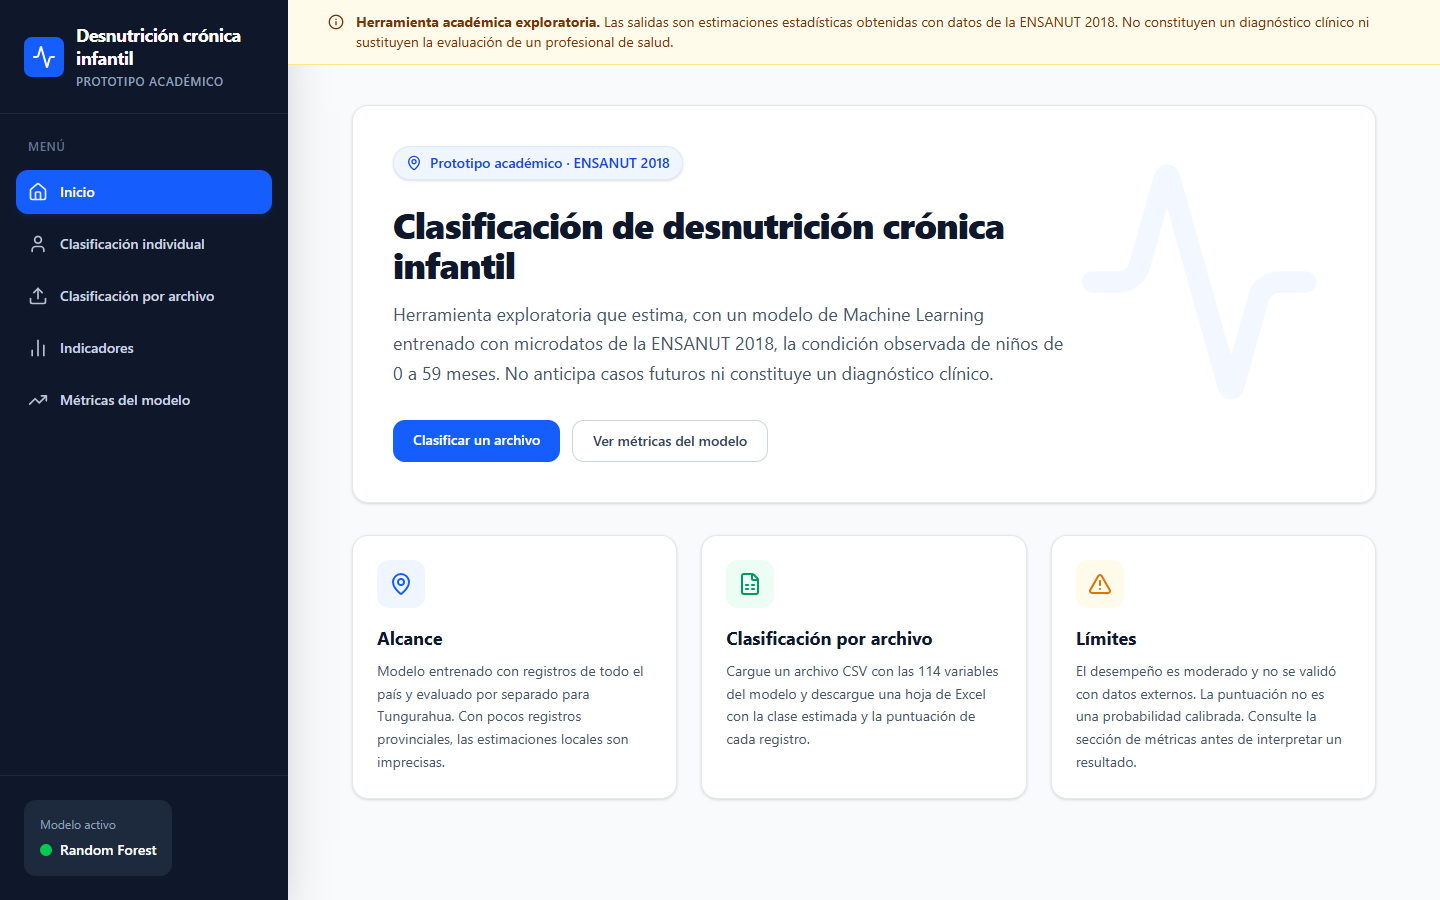
\includegraphics[width=0.85\textwidth]{figuras/ui-inicio.png}
  \caption{Pantalla de inicio del tablero.}
  \label{fig:ui-inicio}
\end{figure}

\section*{B.5 Indicadores}
Muestra, para todo el país o para la provincia elegida en el selector \textit{Ámbito}, los registros de prueba, los casos observados de desnutrición crónica, los que clasifica el modelo y la sensibilidad y la precisión en ese ámbito (Figura~\ref{fig:ui-dashboard}). \textbf{Interpretación:} las cifras se calculan con el conjunto de prueba, es decir, con registros que el modelo no usó para entrenar; no son la prevalencia poblacional, porque la muestra no está ponderada. Cuando el ámbito tiene menos de 150 registros (en Tungurahua, 112), la pantalla advierte que la sensibilidad y la precisión son inestables.

\begin{figure}[H]
  \centering
  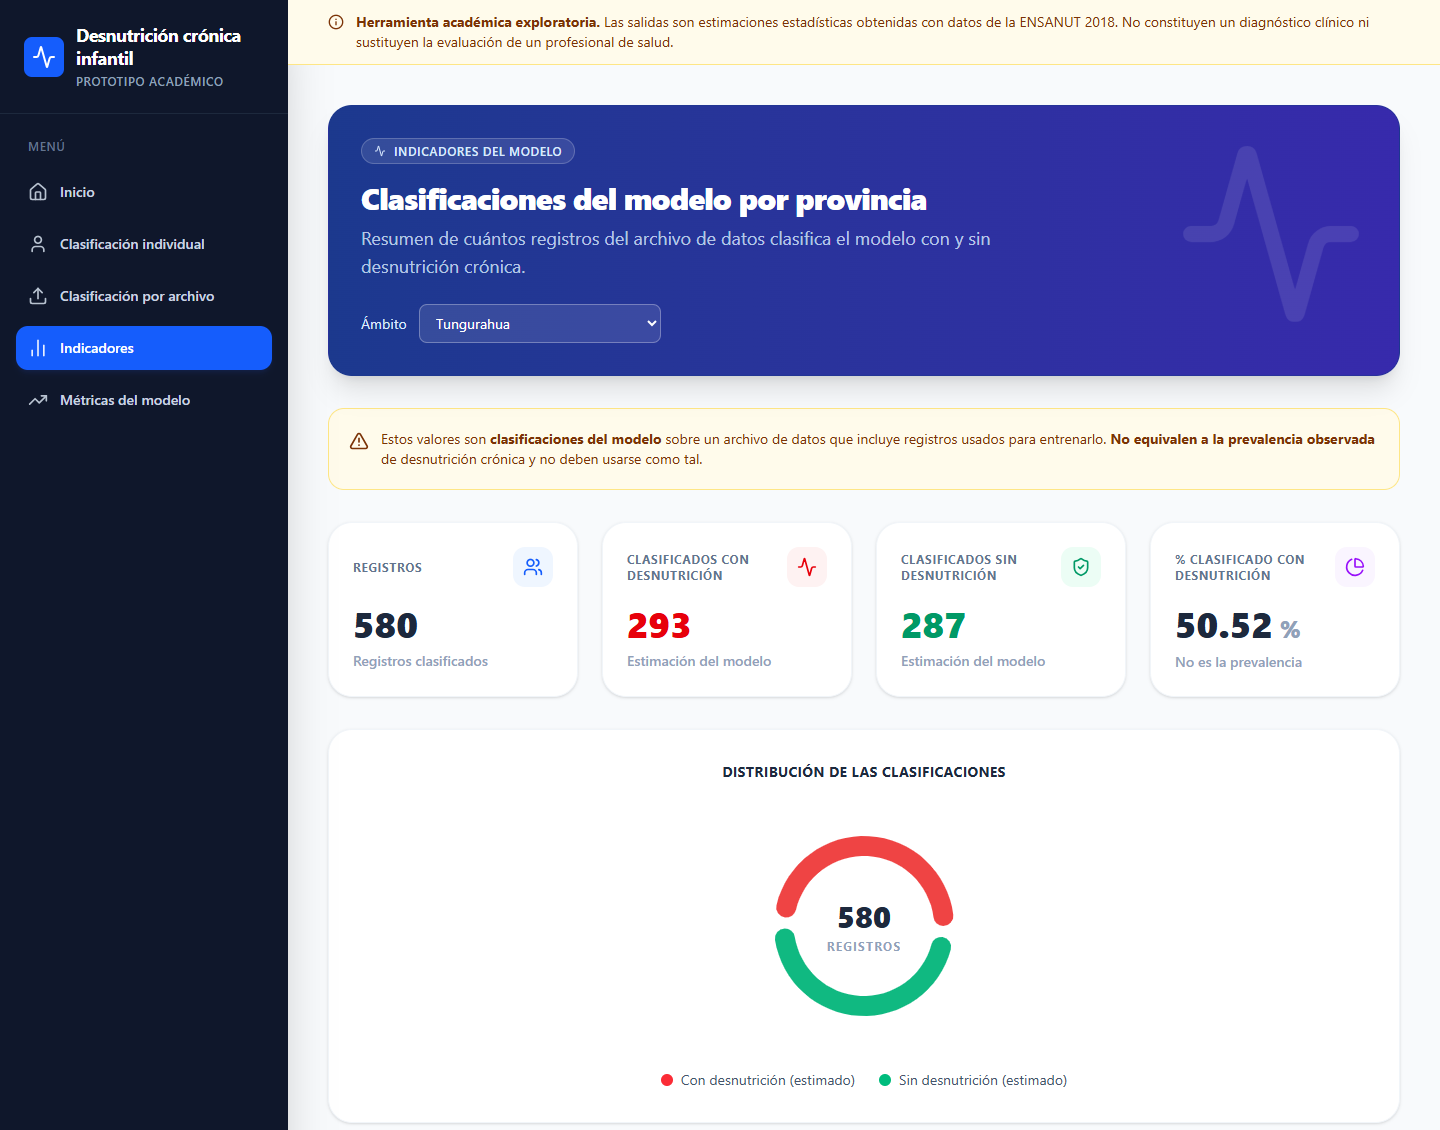
\includegraphics[width=0.85\textwidth]{figuras/ui-dashboard.png}
  \caption{Módulo de indicadores, con el ámbito Tungurahua.}
  \label{fig:ui-dashboard}
\end{figure}

\section*{B.6 Clasificación individual}
El formulario recoge diez datos: edad en meses, sexo, área, provincia, peso y talla al nacer, edad gestacional al nacer, meses de lactancia, y diarrea e infección respiratoria en las dos últimas semanas (Figura~\ref{fig:ui-prediccion}). Las otras 104 variables se envían como nulas y el modelo las completa con la mediana o la moda del entrenamiento. El resultado muestra la clasificación estimada, la puntuación del modelo (no calibrada) y cuántas variables se informaron. \textbf{Uso ilustrativo:} con tan pocos datos la puntuación varía poco (en 512 combinaciones de prueba entre 0.375 y 0.515), por lo que no es interpretable para un niño concreto. Para una clasificación con el modelo evaluado se debe usar la clasificación por archivo.

\begin{figure}[H]
  \centering
  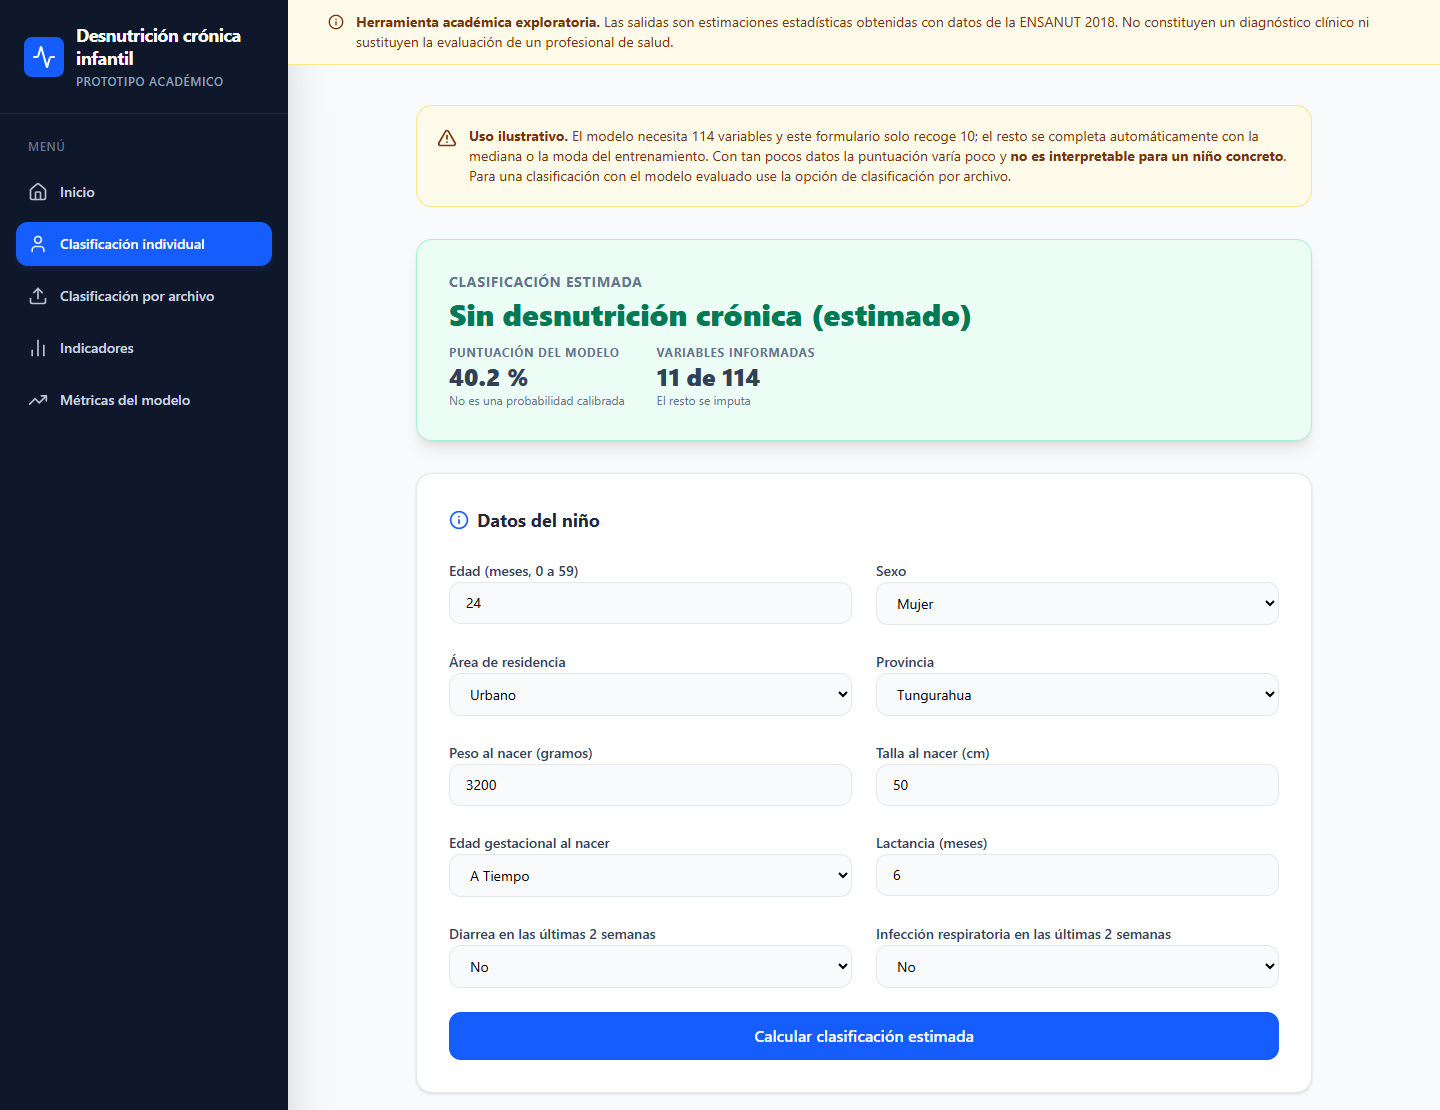
\includegraphics[width=0.85\textwidth]{figuras/ui-prediccion.png}
  \caption{Módulo de clasificación individual con su resultado.}
  \label{fig:ui-prediccion}
\end{figure}

\section*{B.7 Clasificación por archivo}
Pasos (Figura~\ref{fig:ui-masiva}):
\begin{enumerate}
  \item Descargar la plantilla de columnas con el enlace de la pantalla (un CSV solo con el encabezado de las 114 variables).
  \item Completar un niño por fila. Las variables categóricas deben usar las categorías del entrenamiento (Anexo~F).
  \item Seleccionar el archivo (solo formato CSV) y pulsar \textit{Clasificar archivo}.
  \item Se descarga \texttt{resultado\_clasificacion.xlsx} con las columnas originales más \texttt{prediccion} (0 o 1), \texttt{probabilidad} y \texttt{riesgo}.
\end{enumerate}
Si faltan columnas, la pantalla muestra un mensaje y la lista de las faltantes, y no descarga ningún archivo (Figura~\ref{fig:ui-masiva-error}).

\begin{figure}[H]
  \centering
  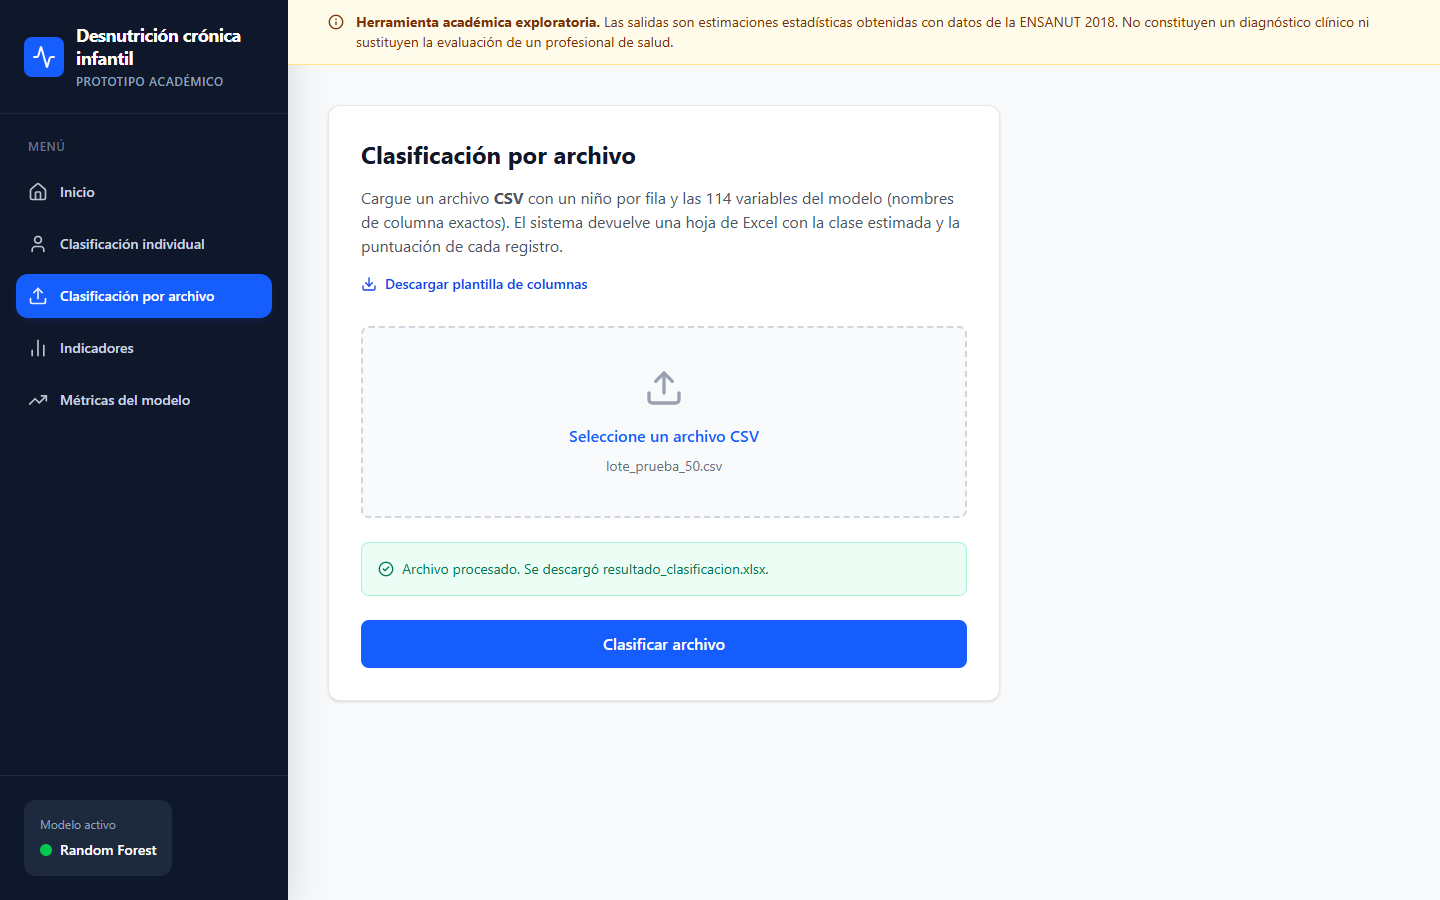
\includegraphics[width=0.85\textwidth]{figuras/ui-masiva.png}
  \caption{Clasificación por archivo: archivo procesado con éxito.}
  \label{fig:ui-masiva}
\end{figure}
\begin{figure}[H]
  \centering
  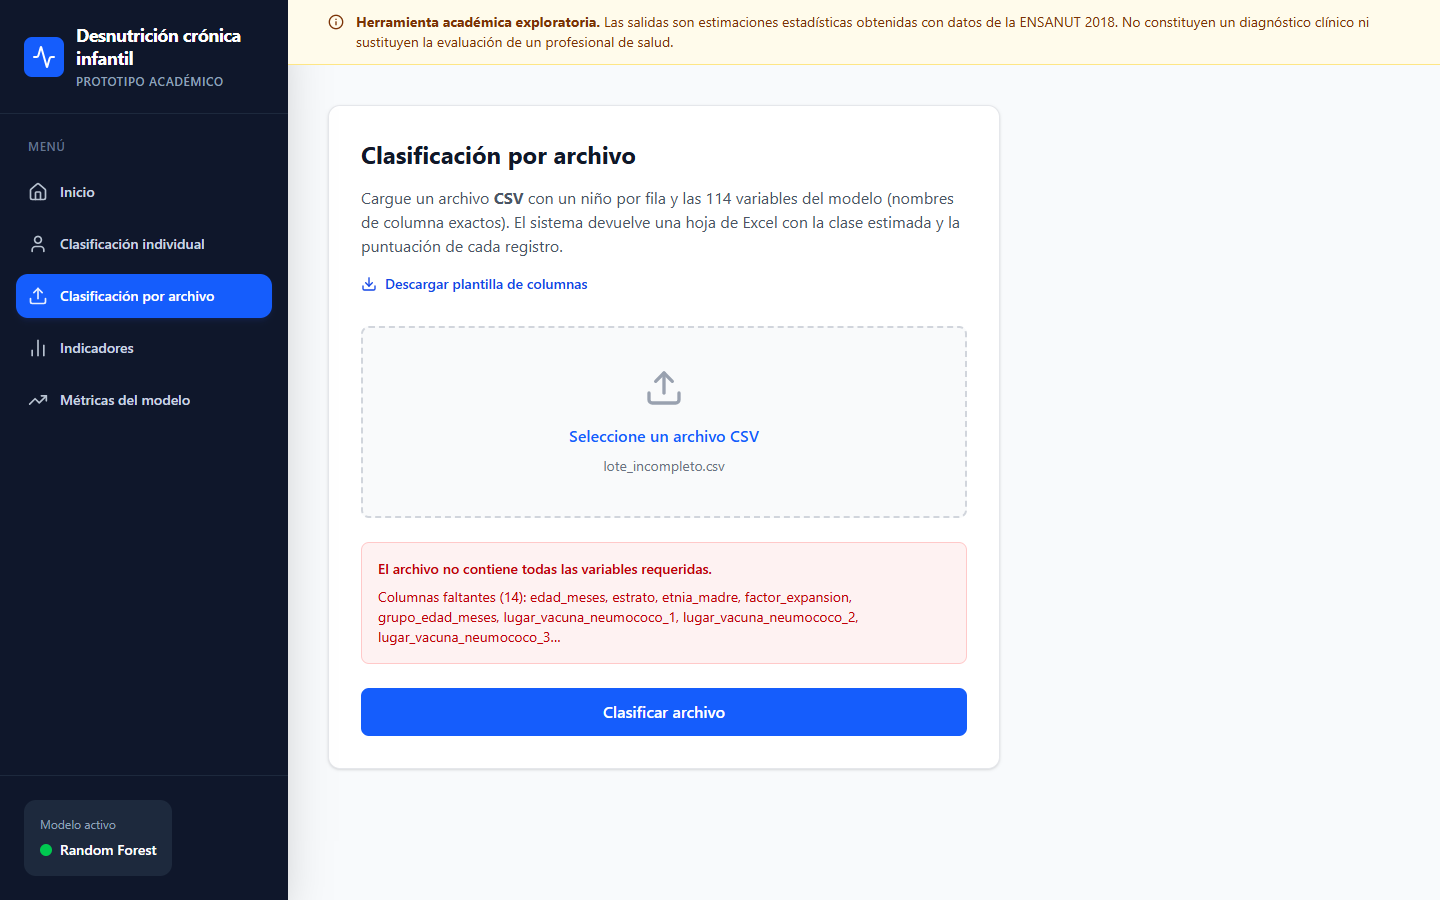
\includegraphics[width=0.85\textwidth]{figuras/ui-masiva-error.png}
  \caption{Clasificación por archivo: mensaje cuando el CSV tiene columnas faltantes.}
  \label{fig:ui-masiva-error}
\end{figure}

\section*{B.8 Métricas del modelo}
Muestra las métricas de la clase con desnutrición crónica en el conjunto de prueba interno (sensibilidad, precisión, F1, exactitud balanceada, ROC-AUC y PR-AUC) y las diez variables más importantes (Figura~\ref{fig:ui-metricas}). Las variables de diseño muestral se marcan en rojo. La importancia no implica causalidad.

\begin{figure}[H]
  \centering
  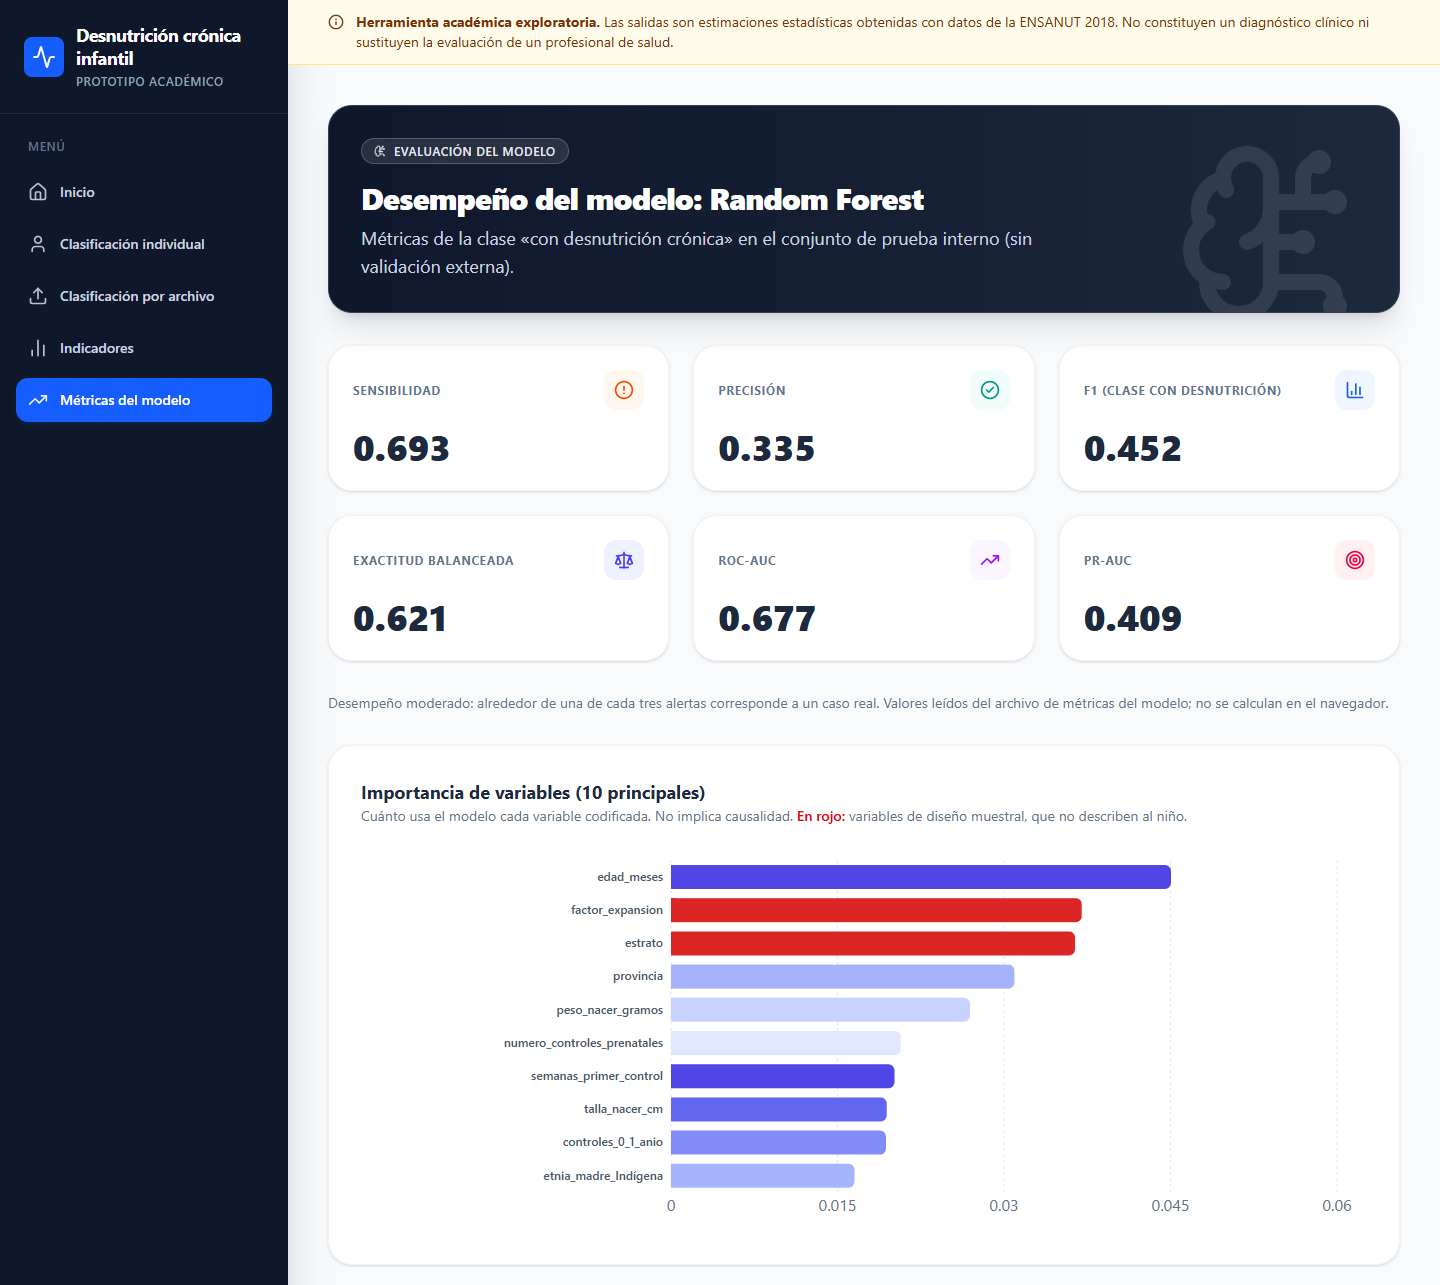
\includegraphics[width=0.85\textwidth]{figuras/ui-metricas.png}
  \caption{Módulo de métricas del modelo.}
  \label{fig:ui-metricas}
\end{figure}

\section*{B.9 Mensajes frecuentes}
\begin{table}[H]
  \caption{Mensajes frecuentes y su causa.}
  \label{tab:mensajes}
  \tablabase\small
  \begin{tabular}{|p{5.0cm}|p{8.4cm}|}
    \hline
    \enc{Mensaje o comportamiento} & \enc{Causa y acción}\\ \hline
    ``El archivo no contiene todas las variables requeridas'' & Faltan columnas en el CSV. Usar la plantilla de columnas\\ \hline
    ``Ocurrió un error al procesar el archivo'' & El archivo no es un CSV válido o tiene categorías no reconocidas. Revisar el formato\\ \hline
    ``API sin conexión'' (barra lateral) & La API no está activa o la dirección configurada es incorrecta\\ \hline
    ``Provincia no válida'' & El ámbito debe elegirse de la lista; la API espera el nombre de la provincia\\ \hline
    Riesgo BAJO con clase estimada positiva (en el Excel) & Ocurría en la versión inicial del servicio; corregido (A.4). Si aparece en un despliegue antiguo, usar la clase\\ \hline
  \end{tabular}
\end{table}

%% ----------------------------------------------------------------- ANEXO C
\anexo{C}{Evidencias de Pruebas del Sistema}

Las pruebas de la API se ejecutaron el 20 de septiembre de 2026 sobre el backend en ejecución local (\textit{TestClient} de FastAPI, modelo v2), con un registro real del conjunto de prueba como entrada. Las pruebas del tablero (CP15 a CP17) se ejecutaron el mismo día en un navegador automatizado (Playwright) sobre la interfaz ya corregida. Además se ejecutaron las 21 pruebas automáticas del repositorio (5 de contrato, 3 del nivel de riesgo, 5 del resumen del tablero y 8 de la lectura de archivos), todas aprobadas.

\begingroup
\scriptsize\setlength{\tabcolsep}{3pt}\arrayrulecolor{black!55}\renewcommand{\arraystretch}{1.1}
\begin{longtable}{|c|p{2.2cm}|p{2.7cm}|p{2.4cm}|p{3.1cm}|c|}
  \caption{Casos de prueba funcional de la API.}
  \label{tab:casos}\\ \hline
  \enc{ID} & \enc{Caso} & \enc{Entrada} & \enc{Esperado} & \enc{Obtenido} & \enc{Estado}\\ \hline
  \endfirsthead
  \tablacont{6}\hline
  \enc{ID} & \enc{Caso} & \enc{Entrada} & \enc{Esperado} & \enc{Obtenido} & \enc{Estado}\\ \hline
  \endhead
  \hline\endfoot
  CP1 & Estado del servicio & \texttt{GET /health} & HTTP 200 y \texttt{OK} & HTTP 200, \texttt{\{"status":"OK"\}} & Pasa\\ \hline
  CP2 & Variables del modelo & \texttt{GET /features} & 114 variables & HTTP 200, 114 variables & Pasa\\ \hline
  CP3 & Información de la API & \texttt{GET /info} & HTTP 200 y modelo activo & HTTP 200, modelo Random Forest & Pasa\\ \hline
  CP4 & Predicción individual & \texttt{POST /predict} con 114 variables & HTTP 200; clase, probabilidad en [0,1] y riesgo & HTTP 200; clase 1, probabilidad 0.437, riesgo MEDIO & Pasa (ver nota)\\ \hline
  CP5 & Variable faltante & \texttt{POST /predict} con 113 variables & HTTP 400 & HTTP 400 & Pasa\\ \hline
  CP6 & Variable sobrante & \texttt{POST /predict} con 115 variables & HTTP 400 & HTTP 400 & Pasa\\ \hline
  CP7 & Cuerpo vacío & \texttt{POST /predict} con \texttt{\{\}} & HTTP 400 & HTTP 400 & Pasa\\ \hline
  CP8 & Predicción masiva & \texttt{POST /predict-file}, CSV de 50 registros & Archivo \texttt{.xlsx} de 50 filas & HTTP 200; \texttt{.xlsx} de 50 filas & Pasa\\ \hline
  CP9 & Resumen nacional & \texttt{GET /dashboard} & HTTP 200 con totales del conjunto de prueba & HTTP 200; \num{3699} registros; 912 observados; \num{1887} clasificados (sensibilidad 0.693) & Pasa (ver nota)\\ \hline
  CP10 & Resumen por provincia & \texttt{GET /dashboard} con provincia Tungurahua & HTTP 200 con totales del conjunto de prueba & HTTP 200; 112 registros; 35 observados; 57 clasificados (sensibilidad 0.686) & Pasa (ver nota)\\ \hline
  CP11 & Métricas del modelo & \texttt{GET /dashboard/}\allowbreak\texttt{metricas} & Valores de \texttt{metricas\_v2.json} & HTTP 200; valores idénticos & Pasa\\ \hline
  CP12 & Importancia de variables & \texttt{GET /dashboard/}\allowbreak\texttt{importancia} & HTTP 200 con lista & HTTP 200; lista de variables & Pasa\\ \hline
  CP13 & Documentación & \texttt{GET /docs} & HTTP 200 & HTTP 200 & Pasa\\ \hline
  CP14 & Archivo Excel en predicción masiva & \texttt{POST /predict-file} con un \texttt{.xlsx} & Resultado o mensaje de error controlado & HTTP 200; \texttt{.xlsx} de 50 filas. Un Excel dañado, un \texttt{.xls} o un archivo vacío devuelven un mensaje de error & Pasa (ver nota)\\ \hline
  CP15 & Formulario individual & 512 combinaciones de los 10 datos, resto nulo (formulario corregido) & Probabilidades que varíen según los datos & Entre 0.375 y 0.515; \SI{85.5}{\percent} con clase 1 (la versión inicial: 0.436--0.512, todas con clase 1) & Falla\\ \hline
  CP16 & Tablero: CSV incompleto & CSV de 5 registros con 100 de 114 columnas & Mensaje claro con columnas faltantes; sin descarga & Mensaje con las columnas faltantes; sin descarga & Pasa\\ \hline
  CP17 & Tablero: CSV válido & CSV de 50 registros del conjunto de prueba & Descarga de \texttt{.xlsx} de 50 filas & \texttt{resultado\_clasificacion.xlsx} con 50 filas y columnas \texttt{prediccion}, \texttt{probabilidad} y \texttt{riesgo} & Pasa\\ \hline
\end{longtable}
\endgroup

\noindent\textbf{Notas.} En CP4, con la versión evaluada inicialmente, la clase asignada (1) y el riesgo (BAJO) no coincidían porque usaban cortes distintos; tras alinear el riesgo con el umbral de 0.42 el caso se volvió a ejecutar y devuelve riesgo MEDIO. Con el servicio corregido, los 50 registros de CP17 son consistentes: 25 con riesgo BAJO (todos clase 0), 21 MEDIO y 4 ALTO (todos clase 1). En la versión evaluada inicialmente, CP9 y CP10 devolvían positivos predichos por el modelo sobre un archivo que incluía los datos de entrenamiento (\num{20510} registros y \num{10626} casos predichos a nivel nacional; 580 registros y 293 casos en Tungurahua), no casos observados. El servicio se corrigió para usar el conjunto de prueba y ambos casos se volvieron a ejecutar: los valores de la tabla son los del servicio corregido y reproducen las métricas de \texttt{metricas\_v2.json} (sensibilidad 0.693 y precisión 0.335). CP14 y CP15 se agregaron al descubrir el comportamiento del servicio de archivos y del formulario. En la versión evaluada inicialmente, CP14 producía una excepción no controlada (\texttt{UnicodeDecodeError}) porque el servicio leía el Excel como CSV; se corrigió (lectura de \texttt{.xlsx} y mensajes de error controlados) y el caso se volvió a ejecutar; CP16 y CP17 verifican la carga de archivos del tablero corregido (Anexo~B).

\noindent\textbf{Resumen.} De los 17 casos, 16 pasan y 1 falla (CP15). Los casos CP1 a CP13 verifican el contrato de la API con datos completos; CP14 verifica el servicio de archivos con Excel (falló en la versión inicial y pasa con el servicio corregido) y CP15 muestra la escasa variación del formulario individual.

\noindent\textbf{Latencia de \texttt{POST /predict}} (100 solicitudes, ejecución local sin red): mediana de 29 ms, percentil 95 de 33 ms y máximo de 38 ms.

\section*{C.1 Ejemplo de solicitud y respuesta (CP4)}
\begin{lstlisting}[frame=single,basicstyle=\ttfamily\footnotesize]
Entrada: registro 0 del conjunto de prueba (114 variables)
Salida : {"prediccion": 1,
          "descripcion": "Con desnutrición crónica",
          "probabilidad": 0.437,
          "riesgo": "MEDIO"}
Cálculo directo sobre el modelo (sin API): 0.437
\end{lstlisting}

\section*{C.2 Pruebas automáticas del repositorio}
\begin{lstlisting}[frame=single,basicstyle=\ttfamily\footnotesize]
$ python -m pytest -q tests
.....................                           [100%]
21 passed
\end{lstlisting}

%% ----------------------------------------------------------------- ANEXO D
\anexo{D}{Trazabilidad entre Objetivos, Métodos y Resultados}

\begin{table}[H]
  \caption{Matriz de trazabilidad.}
  \label{tab:traza}
  \tablabase\scriptsize
  \begin{tabular}{|p{2.6cm}|p{3.1cm}|p{3.6cm}|p{3.5cm}|}
    \hline
    \enc{Objetivo específico} & \enc{Método (capítulo II)} & \enc{Resultado (capítulo III)} & \enc{Conclusión (capítulo IV)}\\ \hline
    1. Analizar y preparar los datos & Fases Obtener, Limpiar y Explorar (Tabla~\ref{tab:osemn}) & Tabla~\ref{tab:datos}; corrección de v1 (Tabla~\ref{tab:v1v2}) & Objetivo 1\\ \hline
    2. Diseñar arquitectura y protocolo & Diseño y requerimientos (Tablas~\ref{tab:rf}, \ref{tab:rnf}) & Tabla~\ref{tab:experimento} & Objetivo 2\\ \hline
    3. Entrenar, comparar y evaluar & Protocolo experimental y métricas & Tablas~\ref{tab:metricas}, \ref{tab:tung}, \ref{tab:sobreajuste}; Figuras~\ref{fig:comparacion}, \ref{fig:matriz}, \ref{fig:curvas} & Objetivo 3\\ \hline
    4. Implementar API y tablero & Contrato de la API (Tabla~\ref{tab:api}) & Tabla~\ref{tab:stack}; Anexos A y B & Objetivo 4\\ \hline
    5. Validar y documentar limitaciones & Pruebas funcionales (Tabla~\ref{tab:tecnicas}) & Anexo C; Tabla~\ref{tab:cumplimiento} & Objetivo 5 y limitaciones\\ \hline
  \end{tabular}
\end{table}

\begin{table}[H]
  \caption{Requerimientos y casos de prueba que los verifican.}
  \label{tab:req-cp}
  \tablabase\small
  \begin{tabular}{|c|p{5.2cm}|p{5.2cm}|}
    \hline
    \enc{Requerimiento} & \enc{Evidencia principal} & \enc{Casos de prueba}\\ \hline
    RF3, RNF1 & Servicio de predicción y validación de entradas & CP4, CP5, CP6, CP7\\ \hline
    RF4 & Predicción masiva & CP8, CP14, CP16, CP17\\ \hline
    RF5 & Métricas del modelo & CP11\\ \hline
    RF6 & Indicadores del tablero & CP9, CP10, CP12\\ \hline
    RF7 & Documentación interactiva & CP13\\ \hline
    RNF2 & Rendimiento & Latencia de 100 solicitudes\\ \hline
    RNF3 & Disponibilidad & CP1, CP3\\ \hline
    RNF7 & Uso responsable & Revisión de la interfaz en todas las pantallas (Anexo~B)\\ \hline
  \end{tabular}
\end{table}

%% ----------------------------------------------------------------- ANEXO E
\anexo{E}{Repositorio de Versionamiento de Código}

\section*{E.1 Repositorios}
El código está en un único repositorio consolidado de GitHub, cuya cuenta propietaria es \texttt{8afer99c}: \url{https://github.com/8afer99c/desnutricion_tesis}. Contiene los notebooks originales, el pipeline corregido (\texttt{pipeline\_v2}), la API y el tablero. Se publicaron dos ramas: \texttt{pipeline-v2-fixes} (rama por defecto del repositorio) y \texttt{main} (rama desplegada). El historial de commits conserva la autoría que Git registró en cada commit.

La versión final del tablero corresponde al commit \texttt{b441664} de \texttt{pipeline-v2-fixes} y a su integración en \texttt{main} (commit \texttt{8df0ade}, 20 de septiembre de 2026). El archivo \texttt{metricas\_v2.json} se versionó en \texttt{45928dd} (\texttt{main}) y \texttt{af4fcf4} (\texttt{pipeline-v2-fixes}), y la corrección del nivel de riesgo de la API está en \texttt{588d8fe} (\texttt{main}) y \texttt{7b37205} (\texttt{pipeline-v2-fixes}). El resumen del tablero con el conjunto de prueba (\texttt{data/test\_v2.csv}) está en \texttt{edf40ae} (\texttt{main}) y \texttt{d785b95} (\texttt{pipeline-v2-fixes}). La lectura controlada de CSV y Excel en \texttt{/predict-file} está en \texttt{89a23d5} (\texttt{main}) y \texttt{db5a77f} (\texttt{pipeline-v2-fixes}). Los notebooks y el paquete \texttt{pipeline\_v2} se conservan en el historial hasta el commit \texttt{1b4b767}, ya que desde el commit \texttt{bf27226} la reorganización del repositorio los retiró del árbol de archivos actual; se recuperan con \texttt{git show <commit>:<ruta>}.

\section*{E.2 Reproducción de los resultados}
Desde la carpeta del proyecto, con Python 3.13 y las versiones de la Tabla~\ref{tab:deps}, el pipeline se ejecuta en este orden:
\begin{lstlisting}[frame=single,basicstyle=\ttfamily\footnotesize]
python -m pipeline_v2.build_clean_dataset   # base sin fuga (18 493)
python -m pipeline_v2.split_dataset         # train_v2 / test_v2
python -m pipeline_v2.leakage_screen        # revision de fuga
python -m pipeline_v2.entrenar_modelo       # modelo_v2 y metricas_v2
python -m pipeline_v2.comparar_v1_v2        # comparacion v1 vs v2
python -m pipeline_v2.tabla_experimento     # tabla unica del experimento
\end{lstlisting}
Los archivos generados quedan en \texttt{pipeline\_v2/output}. Cargar \texttt{modelo\_v2.joblib} requiere la misma versión de scikit-learn con la que se entrenó (1.6.1).

\section*{E.3 Historial de cambios del pipeline corregido}
\begingroup
\scriptsize\setlength{\tabcolsep}{3pt}\arrayrulecolor{black!55}\renewcommand{\arraystretch}{1.1}
\begin{longtable}{|c|c|p{9.8cm}|}
  \caption{Commits principales del repositorio (ramas \texttt{pipeline-v2-fixes} y \texttt{main}).}
  \label{tab:commits}\\ \hline
  \enc{Fecha} & \enc{Commit} & \enc{Descripción}\\ \hline
  \endfirsthead
  \tablacont{3}\hline
  \enc{Fecha} & \enc{Commit} & \enc{Descripción}\\ \hline
  \endhead
  \hline\endfoot
  2026-09-12 & \texttt{7cc7372} & Estructura del paquete \texttt{pipeline\_v2} y entorno de desarrollo\\ \hline
  2026-09-12 & \texttt{46c702d} & Captura de las métricas base del modelo v1\\ \hline
  2026-09-12 & \texttt{b00adf2} & Eliminar filas con variable objetivo sin medir en vez de imputarlas\\ \hline
  2026-09-12 & \texttt{b873079} & Regenerar la partición entrenamiento/prueba limpia y reproducible\\ \hline
  2026-09-12 & \texttt{d711dab} & Revisión automática de fuga por variable\\ \hline
  2026-09-13 & \texttt{2a744f9} & Pipeline de entrenamiento: selección real, desbalance, umbral y métricas por clase\\ \hline
  2026-09-13 & \texttt{f405ca5} & Comparación controlada entre v1 y v2\\ \hline
  2026-09-13 & \texttt{c03200d} & Reportar sobreajuste e hiperparámetros; aislar el preprocesador\\ \hline
  2026-09-13 & \texttt{54cd860} & Aviso sobre los números inflados de v1 y tabla del experimento\\ \hline
  2026-09-13 & \texttt{20f4bde} & Regularizar Random Forest (menor tamaño y sobreajuste)\\ \hline
  2026-09-13 & \texttt{1b4b767} & Incorporar el código de la API y los notebooks al repositorio consolidado\\ \hline
  2026-09-13 & \texttt{bf27226} & Interfaz web y arquitectura estructurada\\ \hline
  2026-09-13 & \texttt{1da04ff} & Variable \texttt{VITE\_API\_URL} para el despliegue en Vercel\\ \hline
  2026-09-20 & \texttt{b441664} & Interfaz académica exploratoria: aviso, métricas v2, formulario con 114 variables y carga CSV corregidos\\ \hline
  2026-09-20 & \texttt{8df0ade} & Integración de \texttt{pipeline-v2-fixes} en \texttt{main} y recompilación de la aplicación web (rama \texttt{main})\\ \hline
  2026-09-20 & \texttt{45928dd}, \texttt{af4fcf4} & Versionar \texttt{metricas\_v2.json} (umbral 0.42 y métricas del modelo v2 en el despliegue)\\ \hline
  2026-09-20 & \texttt{588d8fe}, \texttt{7b37205} & Nivel de riesgo de la API coherente con el umbral de decisión 0.42 (\texttt{main} y \texttt{pipeline-v2-fixes})\\ \hline
  2026-09-20 & \texttt{edf40ae}, \texttt{d785b95} & Resumen del tablero con el conjunto de prueba: casos observados y clasificados, sensibilidad y precisión\\ \hline
  2026-09-20 & \texttt{89a23d5}, \texttt{db5a77f} & Lectura controlada de CSV y Excel en \texttt{/predict-file}, con mensajes de error para archivos inválidos\\ \hline
\end{longtable}
\endgroup

%% ----------------------------------------------------------------- ANEXO F
\anexo{F}{Diccionario de las Variables Predictoras}

La Tabla~\ref{tab:diccionario} describe las 114 variables predictoras en el orden de las columnas del conjunto de datos: tipo, porcentaje de valores ausentes en la base original, rango o categorías principales y etiqueta de la pregunta original de la ENSANUT. La variable objetivo es \texttt{desnutricion\_cronica}. Las categorías se muestran tal como figuran en los datos.

\begingroup
\tiny\setlength{\tabcolsep}{2.5pt}\arrayrulecolor{black!55}\renewcommand{\arraystretch}{1.1}
\begin{longtable}{|r|p{3.1cm}|c|r|p{3.0cm}|p{3.8cm}|}
  \caption{Diccionario de las variables predictoras. \% nulos: porcentaje de valores ausentes en la base original antes de la imputación.}
  \label{tab:diccionario}\\ \hline
  \enc{N.º} & \enc{Variable} & \enc{Tipo} & \enc{\% nulos} & \enc{Rango o categorías} & \enc{Etiqueta original (ENSANUT)} \\ \hline
  \endfirsthead
  \tablacont{6}\hline
  \enc{N.º} & \enc{Variable} & \enc{Tipo} & \enc{\% nulos} & \enc{Rango o categorías} & \enc{Etiqueta original (ENSANUT)} \\ \hline
  \endhead
  \hline\endfoot
  1 & \texttt{area} & Cat. & 0.0 & 2 cat.: Urbano; Rural & Área \\ \hline
  2 & \texttt{provincia} & Num. & 0.0 & 1 a 90 & Provincia \\ \hline
  3 & \texttt{orden\_hijo} & Num. & 0.0 & 1 a 3 & Orden del hijo \\ \hline
  4 & \texttt{sexo} & Cat. & 0.0 & 2 cat.: Hombre; Mujer & Sexo \\ \hline
  5 & \texttt{embarazo\_planeado} & Cat. & 0.0 & 4 cat.: Tener Ese Hijo?; Quería Esperar Mas T; … & 403.  En la época en la que quedó embarazada de (…), quería U… \\ \hline
  6 & \texttt{embarazo\_deseado\_pareja} & Cat. & 0.0 & 4 cat.: Tener Ese Hijo?; Quería Esperar Mas T; … & 405.  ¿Quería su pareja: \\ \hline
  7 & \texttt{control\_prenatal} & Cat. & 0.0 & 2 cat.: Si; No & 406.  ¿Tuvo algún control prenatal cuando estaba embarazada d… \\ \hline
  8 & \texttt{lugar\_control\_prenatal} & Cat. & 4.2 & 10 cat.: Establecimientos De ; Clínica/Consultorio ; … & 407.a ¿Dónde se hizo el control con mayor frecuencia? \\ \hline
  9 & \texttt{consumo\_micronutrientes\_embarazo} & Cat. & 4.2 & 4 cat.: Hierro Más Ácido Fól; Hierro?; … & 408.  ¿Consumió algún micronutriente durante el embarazo como: \\ \hline
  10 & \texttt{frecuencia\_micronutrientes} & Cat. & 6.3 & 3 cat.: Diaria; Pasando Un Día; … & 409.a ¿Con qué frecuencia tomaba Los micronutrientes? \\ \hline
  11 & \texttt{control\_peso\_embarazo} & Cat. & 4.2 & 3 cat.: Si; No; … & 410.  ¿Durante el embarazo le pesaron? \\ \hline
  12 & \texttt{medicion\_altura\_uterina} & Cat. & 4.2 & 3 cat.: Si; No; … & 411.  ¿Durante el embarazo le midieron la barriga? \\ \hline
  13 & \texttt{examen\_vih\_embarazo} & Cat. & 4.2 & 3 cat.: Si; No; … & 412.a ¿Durante el embarazo le hicieron un examen de VIH? \\ \hline
  14 & \texttt{numero\_examenes\_vih} & Num. & 13.3 & 1 a 88 & 412.b Cuántos? \\ \hline
  15 & \texttt{control\_presion\_embarazo} & Cat. & 4.2 & 3 cat.: Si; No; … & 413.  ¿Durante el embarazo ¿le tomaron la presión? \\ \hline
  16 & \texttt{examen\_sangre\_embarazo} & Cat. & 4.2 & 3 cat.: Si; No; … & 414.  ¿Durante el embarazo ¿hicieron un examen de sangre? \\ \hline
  17 & \texttt{examen\_orina\_embarazo} & Cat. & 4.2 & 3 cat.: Si; No; … & 415.  ¿Durante el embarazo ¿hicieron un examen de orina? \\ \hline
  18 & \texttt{examen\_sifilis\_embarazo} & Cat. & 4.2 & 3 cat.: Si; No Sabe / No Respond; … & 416.  ¿Durante el embarazo ¿hicieron un examen de sífilis? \\ \hline
  19 & \texttt{vacuna\_tetanos} & Cat. & 4.2 & 3 cat.: Si; No; … & 417.  ¿Durante el embarazo ¿le vacunaron contra el tétanos? \\ \hline
  20 & \texttt{dosis\_tetanos} & Num. & 13.6 & 1 a 99 & 418.  ¿Cuántas veces le vacunaron contra el tétanos? \\ \hline
  21 & \texttt{consejeria\_embarazo} & Cat. & 4.2 & 3 cat.: Si; No; … & 419.a ¿Durante el control del embarazo, recibió consejería o … \\ \hline
  22 & \texttt{consejeria\_micronutrientes} & Cat. & 4.2 & 3 cat.: Si; No; … & 419.b Uso de micronutrientes (hierro, ácido fólico)? \\ \hline
  23 & \texttt{consejeria\_signos\_alarma} & Cat. & 4.2 & 3 cat.: Si; No; … & 419.c Signos de alarma del embarazo (sangrado vaginal, falta … \\ \hline
  24 & \texttt{consejeria\_higiene\_alimentos} & Cat. & 4.2 & 3 cat.: Si; No; … & 419.d Higiene en preparación de alimentos? \\ \hline
  25 & \texttt{consejeria\_lavado\_manos} & Cat. & 4.2 & 3 cat.: Si; No; … & 419.e Lavado de manos? \\ \hline
  26 & \texttt{consejeria\_anticonceptivos} & Cat. & 4.2 & 3 cat.: Si; No; … & 419.f Métodos anticonceptivos? \\ \hline
  27 & \texttt{consejeria\_apego\_lactancia} & Cat. & 4.2 & 3 cat.: Si; No; … & 419.g El apego inmediato, lactancia en la primera hora de vid… \\ \hline
  28 & \texttt{semanas\_primer\_control} & Num. & 4.2 & 0 a 40 & 420.  ¿Cuántas semanas de embarazo tenía cuando le hicieron e… \\ \hline
  29 & \texttt{numero\_controles\_prenatales} & Num. & 4.2 & 0 a 88 & 421.  En total, ¿cuántos controles tuvo antes del parto? \\ \hline
  30 & \texttt{lugar\_parto} & Cat. & 0.0 & 9 cat.: Establecimientos De ; Clínica/Consultorio ; … & 423.a ¿En que lugar tuvo el parto de (..).? \\ \hline
  31 & \texttt{personal\_parto} & Cat. & 0.0 & 8 cat.: Médico; Obstetriz; … & 424.  ¿Qué persona ó profesional le tendió? \\ \hline
  32 & \texttt{tipo\_parto} & Cat. & 0.0 & 2 cat.: Normal (Vaginal); Césaria & 425.  El parto de (...) fue: \\ \hline
  33 & \texttt{prematuro} & Cat. & 0.0 & 4 cat.: A Tiempo; Prematuro; … & 426.  ¿El nacimiento de (...) fue a los 9 meses o antes de ti… \\ \hline
  34 & \texttt{peso\_registrado\_nacer} & Cat. & 0.0 & 2 cat.: Si; No & 428.  ¿Le pesaron a (…) en el momento de nacer o en los prime… \\ \hline
  35 & \texttt{tamizaje\_neonatal} & Cat. & 0.0 & 2 cat.: Si; No & 429.  ¿Le Realizaron a (…) La prueba del Tamizaje Neonatal (p… \\ \hline
  36 & \texttt{bano\_antes\_24h} & Cat. & 0.0 & 3 cat.: Si; No; … & 430.  ¿Le bañaron a (…) antes de cumplir 24 horas de su nacim… \\ \hline
  37 & \texttt{corte\_oportuno\_cordon} & Cat. & 0.0 & 3 cat.: Si; No sabe; … & 431.  ¿Esperaron al menos un minuto para realizar el corte de… \\ \hline
  38 & \texttt{carne\_salud\_infantil} & Cat. & 0.0 & 3 cat.: Si; Si Le Entregaron Per; … & 432.  Tiene usted el carné de salud infantil o libreta integr… \\ \hline
  39 & \texttt{registro\_curva\_crecimiento} & Cat. & 37.8 & 2 cat.: No; Si & 433.a ENCUESTADOR/A OBSERVE SI EL CARNÉ REGISTRA PUNTOS EN LA… \\ \hline
  40 & \texttt{registro\_talla\_nacer} & Cat. & 37.8 & 2 cat.: Si; No & 434.a ENCUESTADOR/A OBSERVE SI EL CARNÉ REGISTRA: TALLA AL NACER \\ \hline
  41 & \texttt{talla\_nacer\_cm} & Num. & 57.3 & 0.42 a 5000 & 434.b cm \\ \hline
  42 & \texttt{registro\_perimetro\_cefalico} & Cat. & 37.8 & 2 cat.: Si; No & 435.a ENCUESTADOR/A OBSERVE SI EL CARNÉ REGISTRA PERÍMETRO CE… \\ \hline
  43 & \texttt{perimetro\_cefalico\_cm} & Num. & 62.8 & 1 a 2603 & 435.b cm \\ \hline
  44 & \texttt{registro\_peso\_nacer} & Cat. & 37.8 & 2 cat.: Si; No & 436.a ENCUESTADOR/A OBSERVE SI EL CARNÉ REGISTRA:PESO AL NACER \\ \hline
  45 & \texttt{peso\_nacer\_gramos} & Num. & 56.1 & 7 a 9800 & 436.b gramos \\ \hline
  46 & \texttt{peso\_nacer\_reportado} & Cat. & 43.9 & 4 cat.: No sabe; Gramos; … & 437.a ¿Cuánto pesó (…)? \\ \hline
  47 & \texttt{bajo\_peso\_nacer} & Cat. & 63.8 & 3 cat.: No sabe; No; … & 438.  ¿(…) Peso menos de 5.5 Libras, 2.5 Kilogramos o 2500 gr… \\ \hline
  48 & \texttt{tamano\_recien\_nacido} & Cat. & 0.0 & 5 cat.: Igual; Más Grande; … & 439.  En comparación con otros niños recién nacidos, ¿cómo co… \\ \hline
  49 & \texttt{control\_posparto} & Cat. & 0.0 & 2 cat.: Si; No & 440.  ¿Tuvo usted algún control después del parto de (...)? \\ \hline
  50 & \texttt{tiempo\_primer\_control\_posparto} & Num. & 38.3 & 0 a 45 & 441.a ¿Cuánto tiempo después del parto de (...) tuvo su prime… \\ \hline
  51 & \texttt{lugar\_control\_posparto} & Cat. & 38.3 & 10 cat.: Establecimientos De ; Clínica/Consultorio ; … & 442.  ¿Dónde tuvo el control de post parto? \\ \hline
  52 & \texttt{control\_medico\_nino} & Cat. & 0.0 & 2 cat.: Si; No & 448.  ¿Después de que nació (...), le llevó para control médico? \\ \hline
  53 & \texttt{tiempo\_primer\_control\_nino} & Num. & 4.1 & 0 a 77 & 449.  ¿Qué tiempo después de nacido (…), le llevó al control … \\ \hline
  54 & \texttt{motivo\_control\_nino} & Cat. & 4.1 & 3 cat.: ¿Para Control Niño S; ¿Estaba Enfermo?; … & 450.  ¿Porqué o para qué le llevó a (…): \\ \hline
  55 & \texttt{controles\_0\_1\_anio} & Num. & 16.6 & 0 a 88 & 451.a ¿De 0 a menos de 1 años ? \\ \hline
  56 & \texttt{controles\_1\_2\_anios} & Num. & 16.6 & 0 a 88 & 451.b ¿De 1 año a menos de 2 años ? \\ \hline
  57 & \texttt{controles\_2\_5\_anios} & Num. & 16.6 & 0 a 99 & 451.c ¿De 2 años a menos de 5 años ? \\ \hline
  58 & \texttt{numero\_controles\_carnet} & Num. & 16.6 & 0 a 24 & 451.a N° de controles en el carnet Último nacido vivo \\ \hline
  59 & \texttt{establecimiento\_salud} & Cat. & 4.1 & 10 cat.: Establecimientos De ; Clínica/Consultorio ; … & 452.  ¿A qué establecimiento o proveedor de salud llevó a (…)? \\ \hline
  60 & \texttt{consejeria\_lactancia} & Cat. & 4.1 & 3 cat.: Si; No; … & 453.a ¿Durante el control del niño, recibió consejería/asesor… \\ \hline
  61 & \texttt{consejeria\_micronutrientes\_nino} & Cat. & 4.1 & 3 cat.: Si; No; … & 453.b Uso de micronutrientes? \\ \hline
  62 & \texttt{consejeria\_alimentacion\_complementaria} & Cat. & 4.1 & 3 cat.: Si; No; … & 453.c Alimentación complementaria? \\ \hline
  63 & \texttt{consejeria\_higiene\_nino} & Cat. & 4.1 & 3 cat.: Si; No; … & 453.d Higiene en preparación de alimentos? \\ \hline
  64 & \texttt{consejeria\_lavado\_manos\_nino} & Cat. & 4.1 & 3 cat.: Si; No; … & 453.e Lavado de manos? \\ \hline
  65 & \texttt{consejeria\_anticonceptivos\_nino} & Cat. & 4.1 & 3 cat.: Si; No; … & 453.f Métodos anticonceptivos? \\ \hline
  66 & \texttt{consejeria\_desarrollo\_infantil} & Cat. & 4.1 & 3 cat.: Si; No; … & 453.g Desarrollo del niño? \\ \hline
  67 & \texttt{lactancia\_anios} & Num. & 0.0 & 0 a 77 & 454.  ¿Hasta que edad le dio el seno (leche materna) a (..)?:… \\ \hline
  68 & \texttt{lactancia\_meses} & Num. & 0.0 & 0 a 77 & 454.  ¿Hasta que edad le dio el seno (leche materna) a (..)?:… \\ \hline
  69 & \texttt{lactancia\_dias} & Num. & 0.0 & 0 a 77 & 454.  ¿Hasta que edad le dio el seno (leche materna) a (..)?:… \\ \hline
  70 & \texttt{nino\_vive} & Cat. & 0.0 & 1 cat.: Si & 455.  SEÑOR ENCUESTADOR: VEA PREGUNTA 402 ¿Está vivo? \\ \hline
  71 & \texttt{vive\_con\_madre} & Cat. & 0.0 & 2 cat.: Si; No & 456.  ¿Vive (…), con usted actualmente? \\ \hline
  72 & \texttt{diarrea\_ultimas\_2\_semanas} & Cat. & 0.6 & 3 cat.: No; Si; … & 457.  ¿Ha tenido diarrea (…) en las ultimas dos semanas (incl… \\ \hline
  73 & \texttt{infeccion\_respiratoria\_2\_semanas} & Cat. & 0.6 & 2 cat.: No; Si & 473.  ¿En las últimas dos semanas ha tenido (...),tos, moquer… \\ \hline
  74 & \texttt{desparasitacion\_6\_meses} & Cat. & 0.6 & 2 cat.: No; Si & 482.  ¿Le dio a (…) algún desparasitante durante los últimos … \\ \hline
  75 & \texttt{hierro\_polvo\_12\_meses} & Cat. & 0.6 & 2 cat.: No; Si & 483.  En los últimos 12 meses, (…) Recibió del personal de Sa… \\ \hline
  76 & \texttt{hierro\_otra\_presentacion} & Cat. & 0.6 & 2 cat.: No; Si & 485.  En los últimos 12 meses, (…) Recibió del personal de sa… \\ \hline
  77 & \texttt{vitamina\_a\_12\_meses} & Cat. & 0.6 & 2 cat.: No; Si & 486.  En los últimos 12 meses, (…) Recibió del personal salud… \\ \hline
  78 & \texttt{vacuna\_bcg\_carnet} & Cat. & 23.8 & 2 cat.: Si; No & 487.1 BCG - según carnet, tiene dosís? \\ \hline
  79 & \texttt{vacuna\_hepatitis\_b\_carnet} & Cat. & 23.7 & 2 cat.: Si; No & 487.2 HEPATITIS B - según carnet, tiene dosís? \\ \hline
  80 & \texttt{vacuna\_rotavirus\_1\_carnet} & Cat. & 23.7 & 2 cat.: Si; No & 487.3 ROTAVIRUS 1 - según carnet, tiene dosís? \\ \hline
  81 & \texttt{vacuna\_rotavirus\_2\_carnet} & Cat. & 23.7 & 2 cat.: Si; No & 487.4 ROTAVIRUS 2 - según carnet, tiene dosís? \\ \hline
  82 & \texttt{vacuna\_pentavalente\_1\_carnet} & Cat. & 23.7 & 2 cat.: Si; No & 487.5 PENTAVALENTE 1 - según carnet, tiene dosís? \\ \hline
  83 & \texttt{vacuna\_pentavalente\_2\_carnet} & Cat. & 23.7 & 2 cat.: Si; No & 487.6 PENTAVALENTE 2 - según carnet, tiene dosís? \\ \hline
  84 & \texttt{vacuna\_pentavalente\_3\_carnet} & Cat. & 23.7 & 2 cat.: Si; No & 487.7 PENTAVALENTE 3 - según carnet, tiene dosís? \\ \hline
  85 & \texttt{vacuna\_ipv\_1\_carnet} & Cat. & 23.7 & 2 cat.: Si; No & 487.7 IPV 1 - según carnet, tiene dosís? \\ \hline
  86 & \texttt{vacuna\_opv\_2\_carnet} & Cat. & 23.7 & 2 cat.: Si; No & 487.9 OPV 2 - según carnet, tiene dosís? \\ \hline
  87 & \texttt{vacuna\_opv\_3\_carnet} & Cat. & 23.7 & 2 cat.: Si; No & 487.10 OPV 3 - según carnet, tiene dosís? \\ \hline
  88 & \texttt{vacuna\_neumococo\_1\_carnet} & Cat. & 23.7 & 2 cat.: Si; No & 487.11 NEUMOCOCO CJ 1 - según carnet, tiene dosís? \\ \hline
  89 & \texttt{vacuna\_neumococo\_2\_carnet} & Cat. & 23.7 & 2 cat.: Si; No & 487.12 NEUMOCOCO CJ 2 - según carnet, tiene dosís? \\ \hline
  90 & \texttt{vacuna\_neumococo\_3\_carnet} & Cat. & 23.7 & 2 cat.: Si; No & 487.13 NEUMOCOCO CJ 3 - según carnet, tiene dosís? \\ \hline
  91 & \texttt{vacuna\_srp\_1\_carnet} & Cat. & 23.7 & 2 cat.: Si; No & 487.14 SRP 1 - según carnet, tiene dosís? \\ \hline
  92 & \texttt{vacuna\_srp\_2\_carnet} & Cat. & 23.7 & 2 cat.: No; Si & 487.15 SRP 2 - según carnet, tiene dosís? \\ \hline
  93 & \texttt{lugar\_vacuna\_bcg} & Cat. & 0.6 & 12 cat.: Establecimientos De ; No Sabe/ No Responde; … & 487.A1 BCG - Recibió en el: \\ \hline
  94 & \texttt{lugar\_vacuna\_hepatitis\_b} & Cat. & 0.6 & 12 cat.: Establecimientos De ; Aún No La Recibe; … & 487.A2 HEPATITIS B - Recibió en el: \\ \hline
  95 & \texttt{lugar\_vacuna\_rotavirus\_1} & Cat. & 0.6 & 12 cat.: Establecimientos De ; Aún No La Recibe; … & 487.A3 ROTAVIRUS 1 - Recibió en el: \\ \hline
  96 & \texttt{lugar\_vacuna\_rotavirus\_2} & Cat. & 0.6 & 12 cat.: Establecimientos De ; Aún No La Recibe; … & 487.A4 ROTAVIRUS 2 - Recibió en el: \\ \hline
  97 & \texttt{lugar\_vacuna\_pentavalente\_1} & Cat. & 0.6 & 12 cat.: Establecimientos De ; Aún No La Recibe; … & 487.A5 PENTAVALENTE 1 - Recibió en el: \\ \hline
  98 & \texttt{lugar\_vacuna\_pentavalente\_2} & Cat. & 0.6 & 12 cat.: Establecimientos De ; Aún No La Recibe; … & 487.A6 PENTAVALENTE 2 - Recibió en el: \\ \hline
  99 & \texttt{lugar\_vacuna\_pentavalente\_3} & Cat. & 0.6 & 12 cat.: Establecimientos De ; Aún No La Recibe; … & 487.A7 PENTAVALENTE 3 - Recibió en el: \\ \hline
  100 & \texttt{lugar\_vacuna\_ipv\_1} & Cat. & 0.6 & 12 cat.: Establecimientos De ; Aún No La Recibe; … & 487.A8 IPV 1 - Recibió en el: \\ \hline
  101 & \texttt{lugar\_vacuna\_opv\_2} & Cat. & 0.6 & 12 cat.: Establecimientos De ; Aún No La Recibe; … & 487.A9 OPV 2 - Recibió en el: \\ \hline
  102 & \texttt{lugar\_vacuna\_opv\_3} & Cat. & 0.6 & 12 cat.: Establecimientos De ; Aún No La Recibe; … & 487.A10 OPV 3 - Recibió en el: \\ \hline
  103 & \texttt{lugar\_vacuna\_neumococo\_1} & Cat. & 0.6 & 12 cat.: Establecimientos De ; Aún No La Recibe; … & 487.A11 NEUMOCOCO CJ 1 - Recibió en el: \\ \hline
  104 & \texttt{lugar\_vacuna\_neumococo\_2} & Cat. & 0.6 & 12 cat.: Establecimientos De ; Aún No La Recibe; … & 487.A12 NEUMOCOCO CJ 2 - Recibió en el: \\ \hline
  105 & \texttt{lugar\_vacuna\_neumococo\_3} & Cat. & 0.7 & 12 cat.: Establecimientos De ; Aún No La Recibe; … & 487.A13 NEUMOCOCO CJ 3 - Recibió en el: \\ \hline
  106 & \texttt{lugar\_vacuna\_srp\_1} & Cat. & 0.7 & 12 cat.: Establecimientos De ; Aún No La Recibe; … & 487.A14 SRP 1 - Recibió en el: \\ \hline
  107 & \texttt{lugar\_vacuna\_srp\_2} & Cat. & 0.7 & 12 cat.: Establecimientos De ; Aún No La Recibe; … & 487.A15 SRP 2 - Recibió en el: \\ \hline
  108 & \texttt{region\_madre} & Cat. & 0.0 & 4 cat.: Sierra; Costa; … & Región de la mef \\ \hline
  109 & \texttt{etnia\_madre} & Cat. & 0.0 & 5 cat.: Mestizo; Indígena; … & Identificación étnica de la mef \\ \hline
  110 & \texttt{edad\_meses} & Num. & 0.0 & 0 a 59 & Edad en meses \\ \hline
  111 & \texttt{grupo\_edad\_meses} & Cat. & 0.0 & 8 cat.: 48-59; 0-11; … & Grupo edad en meses \\ \hline
  112 & \texttt{nivel\_instruccion\_madre} & Cat. & 0.0 & 4 cat.: Educación Media/Bach; Educación Básica; … & Nivel de instrucción de la mef \\ \hline
  113 & \texttt{factor\_expansion} & Num. & 0.0 & 2.862 a 1403 & Factor de expansión \\ \hline
  114 & \texttt{estrato} & Num. & 0.0 & 111 a 9023 & Estratos \\ \hline
\end{longtable}
\endgroup


%% ----------------------------------------------------------------- ANEXO G
\anexo{G}{Perfil de los Datos}

\section*{G.1 Valores nulos}
La Figura~\ref{fig:nulos} muestra las 25 variables con mayor porcentaje de valores ausentes en la base original (calculado sobre los \num{18493} registros del modelo). De los 114 predictores, 84 tenían algún valor ausente, 32 superaban el \SI{10}{\percent}, 11 el \SI{30}{\percent} y 4 el \SI{50}{\percent}. La base de modelado no contiene nulos: se imputaron en la limpieza inicial, sobre todos los registros y antes de la partición. El notebook \texttt{LIMPIEZA.ipynb}, recuperado del historial del repositorio (commit \texttt{1b4b767}), muestra la regla: moda para las variables categóricas y mediana para las numéricas, calculadas sobre la base completa. Ese notebook imputaba también con la mediana la variable objetivo, el factor de expansión y el estrato; el pipeline corregido elimina, en lugar de imputar, los registros con variable objetivo sin medir. El Anexo~F indica el porcentaje original de nulos de cada variable.

\begin{figure}[H]
  \centering
  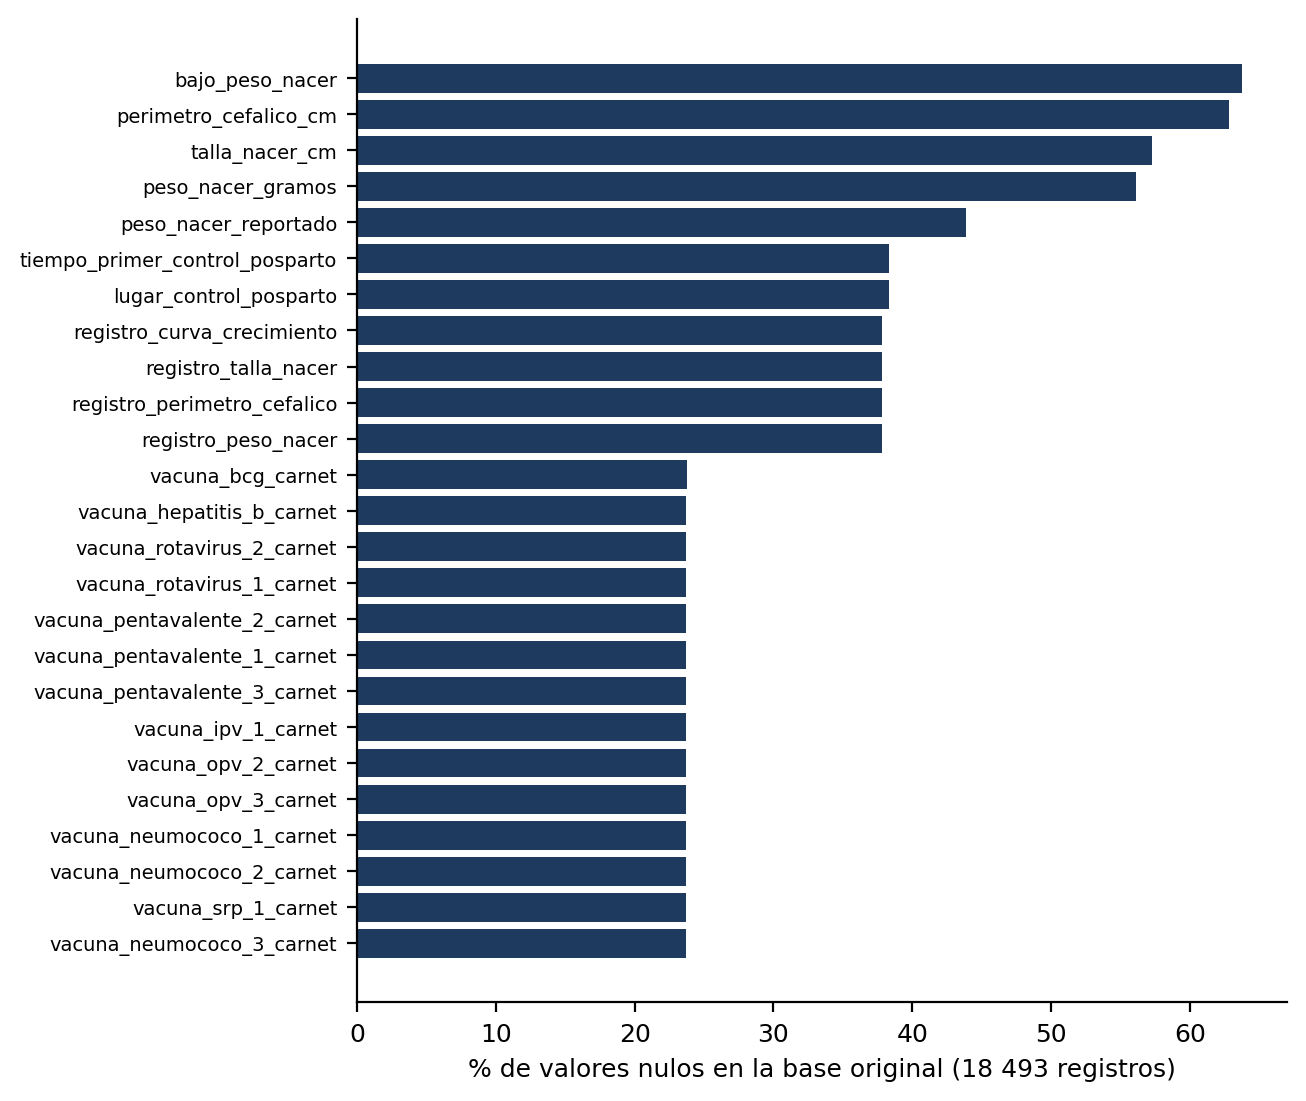
\includegraphics[width=0.8\textwidth]{figuras/anexo-nulos.png}
  \caption{Variables predictoras con mayor porcentaje de valores ausentes en la base original. Elaboración propia.}
  \label{fig:nulos}
\end{figure}

\section*{G.2 Distribución de variables numéricas}
\begin{figure}[H]
  \centering
  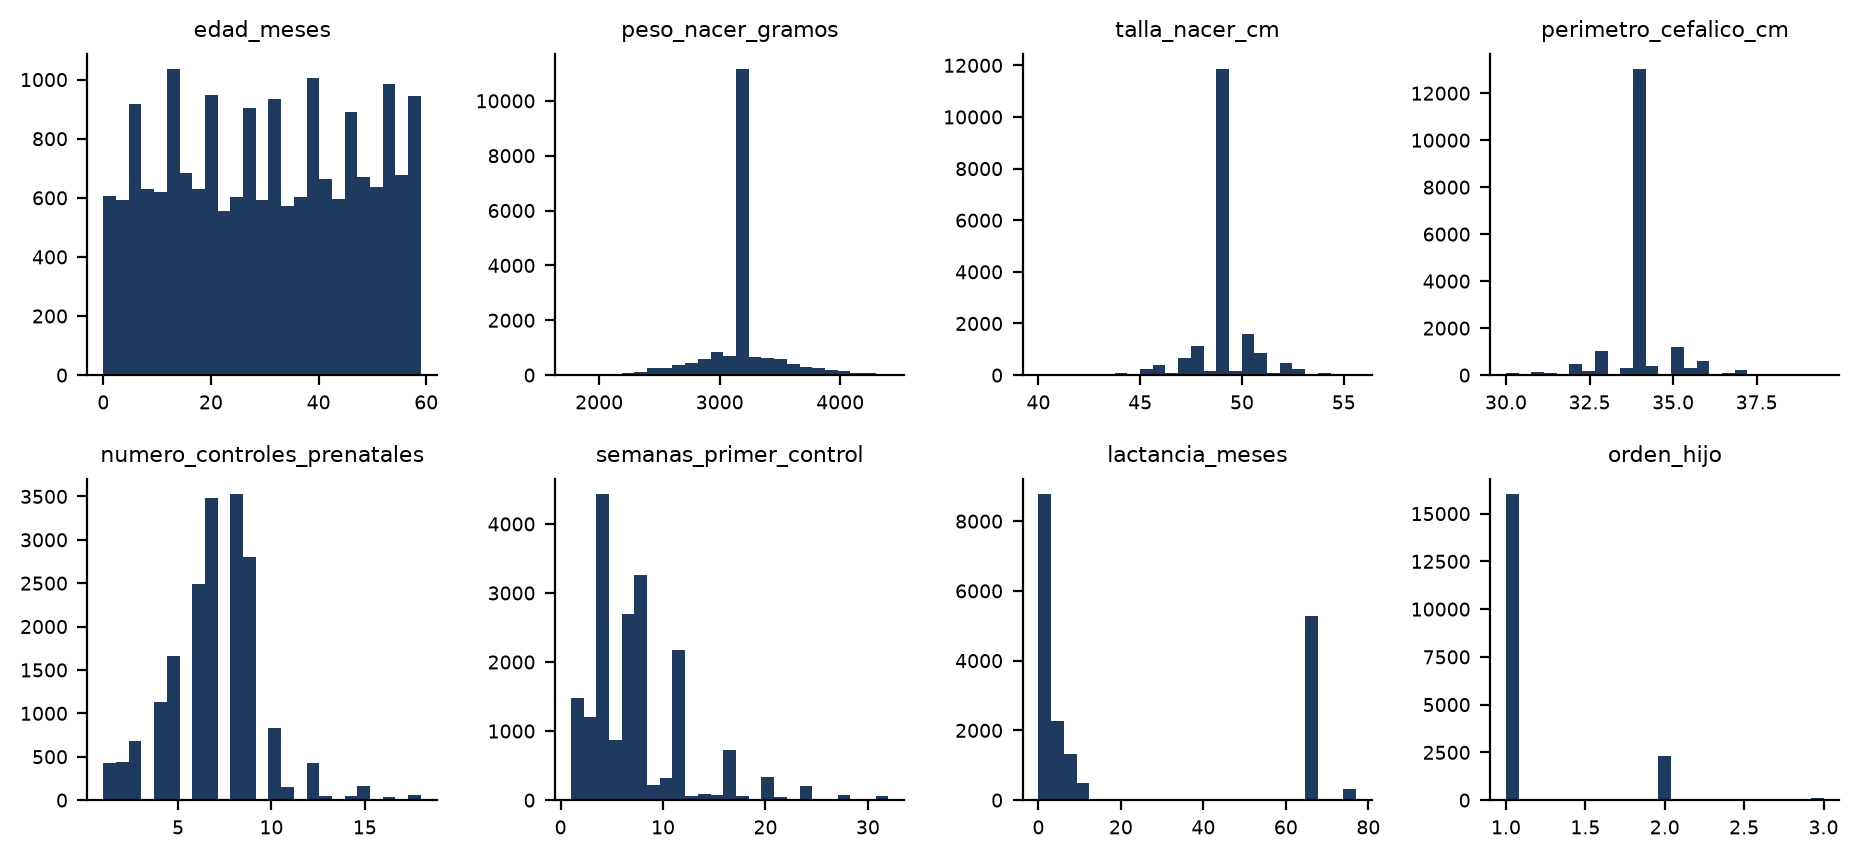
\includegraphics[width=\textwidth]{figuras/anexo-histogramas.png}
  \caption{Histogramas de variables numéricas seleccionadas (sin el 0.5\,\% de valores extremos en cada cola). Elaboración propia.}
  \label{fig:histogramas}
\end{figure}

\section*{G.3 Prevalencia por categoría}
La Figura~\ref{fig:prevcat} muestra la prevalencia muestral de desnutrición crónica según variables categóricas seleccionadas (categorías con al menos 30 registros; la línea roja indica la prevalencia global de \SI{24.7}{\percent}) y la Tabla~\ref{tab:prevcat} los valores. Son prevalencias sin ponderar y asociaciones descriptivas, no efectos causales.

\begin{figure}[H]
  \centering
  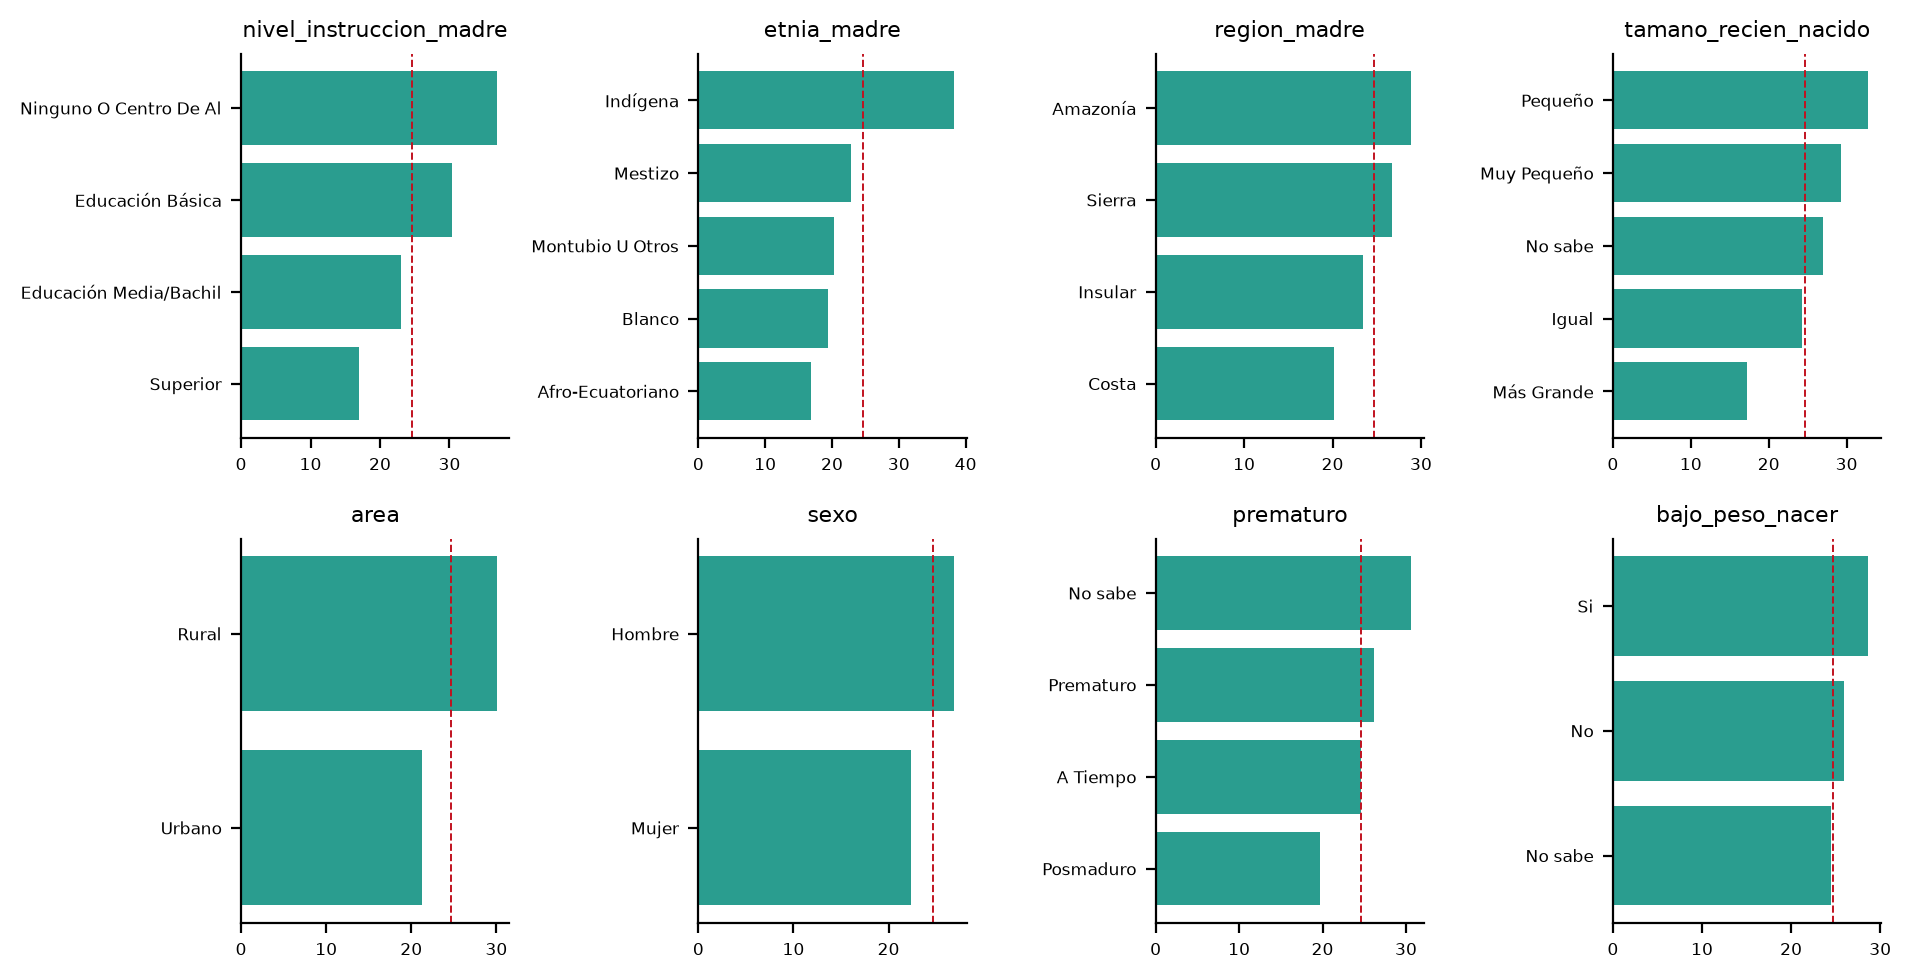
\includegraphics[width=\textwidth]{figuras/anexo-prevalencia-categorias.png}
  \caption{Prevalencia muestral de desnutrición crónica por categoría. Elaboración propia.}
  \label{fig:prevcat}
\end{figure}

\begingroup
\scriptsize\setlength{\tabcolsep}{4pt}\arrayrulecolor{black!55}\renewcommand{\arraystretch}{1.1}
\begin{longtable}{|p{4.4cm}|p{5.6cm}|r|r|}
  \caption{Prevalencia muestral de desnutrición crónica por categoría (sin ponderar).}
  \label{tab:prevcat}\\ \hline
  \enc{Variable} & \enc{Categoría} & \enc{n} & \enc{Prevalencia (\%)} \\ \hline
  \endfirsthead
  \tablacont{4}\hline
  \enc{Variable} & \enc{Categoría} & \enc{n} & \enc{Prevalencia (\%)} \\ \hline
  \endhead
  \hline\endfoot
    \texttt{nivel\_instruccion\_madre} & Superior & 3710 & 17.0 \\ \hline
    \texttt{nivel\_instruccion\_madre} & Educación Media/Bachillerato & 7864 & 23.0 \\ \hline
    \texttt{nivel\_instruccion\_madre} & Educación Básica & 6696 & 30.4 \\ \hline
    \texttt{nivel\_instruccion\_madre} & Ninguno O Centro De Alfabetización & 223 & 36.8 \\ \hline
    \texttt{etnia\_madre} & Afro-Ecuatoriano & 756 & 16.8 \\ \hline
    \texttt{etnia\_madre} & Blanco & 226 & 19.5 \\ \hline
    \texttt{etnia\_madre} & Montubio U Otros & 805 & 20.2 \\ \hline
    \texttt{etnia\_madre} & Mestizo & 14056 & 22.9 \\ \hline
    \texttt{etnia\_madre} & Indígena & 2650 & 38.2 \\ \hline
    \texttt{region\_madre} & Costa & 6991 & 20.1 \\ \hline
    \texttt{region\_madre} & Insular & 371 & 23.5 \\ \hline
    \texttt{region\_madre} & Sierra & 7014 & 26.7 \\ \hline
    \texttt{region\_madre} & Amazonía & 4117 & 28.9 \\ \hline
    \texttt{tamano\_recien\_nacido} & Más Grande & 3267 & 17.2 \\ \hline
    \texttt{tamano\_recien\_nacido} & Igual & 10770 & 24.3 \\ \hline
    \texttt{tamano\_recien\_nacido} & No sabe & 946 & 27.0 \\ \hline
    \texttt{tamano\_recien\_nacido} & Muy Pequeño & 796 & 29.3 \\ \hline
    \texttt{tamano\_recien\_nacido} & Pequeño & 2714 & 32.8 \\ \hline
    \texttt{area} & Urbano & 11240 & 21.2 \\ \hline
    \texttt{area} & Rural & 7253 & 30.0 \\ \hline
    \texttt{sexo} & Mujer & 8981 & 22.3 \\ \hline
    \texttt{sexo} & Hombre & 9512 & 26.9 \\ \hline
    \texttt{prematuro} & Posmaduro & 442 & 19.7 \\ \hline
    \texttt{prematuro} & A Tiempo & 15853 & 24.6 \\ \hline
    \texttt{prematuro} & Prematuro & 2149 & 26.2 \\ \hline
    \texttt{prematuro} & No sabe & 49 & 30.6 \\ \hline
    \texttt{bajo\_peso\_nacer} & No sabe & 17001 & 24.5 \\ \hline
    \texttt{bajo\_peso\_nacer} & No & 920 & 26.0 \\ \hline
    \texttt{bajo\_peso\_nacer} & Si & 572 & 28.7 \\ \hline
\end{longtable}
\endgroup


%% ----------------------------------------------------------------- ANEXO H
\anexo{H}{Resultados Ampliados}

\section*{H.1 Modelos base: matrices de confusión}
\begin{table}[H]
  \caption{Conteos de la matriz de confusión de los modelos base (clase 1 = con desnutrición crónica).}
  \label{tab:conf4}
  \tablabase\footnotesize
  \begin{tabular}{|l|c|c|c|c|c|}
    \hline
    \enc{Modelo} & \enc{Umbral} & \enc{VP} & \enc{FN} & \enc{FP} & \enc{VN} \\ \hline
    Regresión logística & 0.50 & 557 & 355 & 994 & 1793 \\ \hline
    Regresión logística & 0.47 & 614 & 298 & 1187 & 1600 \\ \hline
    Árbol de decisión & 0.50 & 274 & 638 & 634 & 2153 \\ \hline
    Árbol de decisión & 0.05 & 274 & 638 & 634 & 2153 \\ \hline
    Random Forest & 0.50 & 23 & 889 & 11 & 2776 \\ \hline
    Random Forest & 0.23 & 670 & 242 & 1336 & 1451 \\ \hline
    XGBoost & 0.50 & 385 & 527 & 634 & 2153 \\ \hline
    XGBoost & 0.24 & 747 & 165 & 1787 & 1000 \\ \hline
  \end{tabular}
\end{table}


\begin{figure}[H]
  \centering
  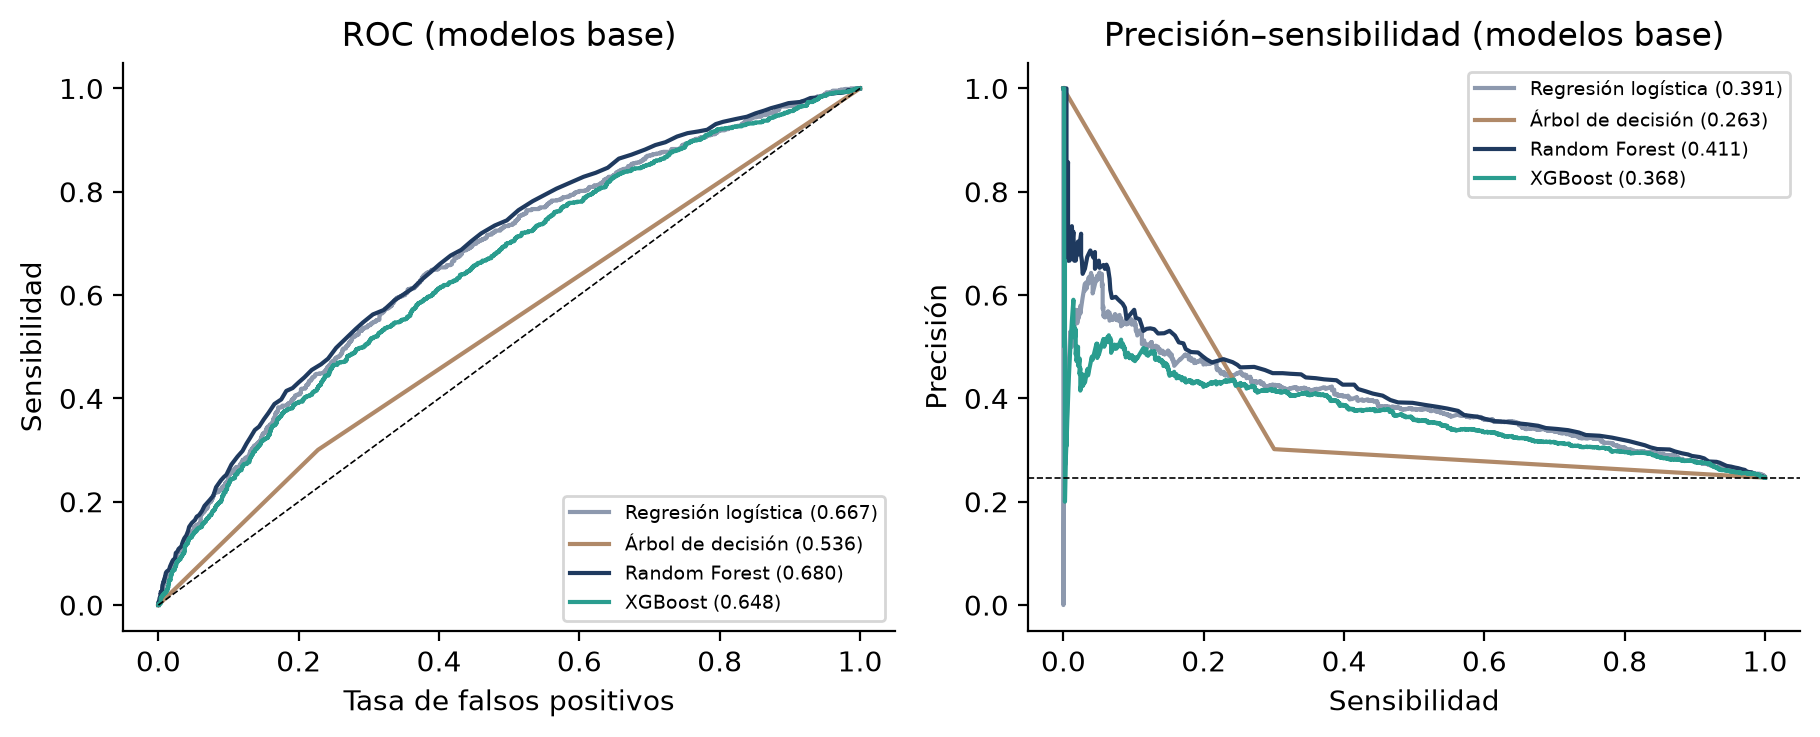
\includegraphics[width=\textwidth]{figuras/anexo-curvas-4modelos.png}
  \caption{Curvas ROC y de precisión--sensibilidad de los cuatro modelos base en el conjunto de prueba. Elaboración propia.}
  \label{fig:curvas4}
\end{figure}

\section*{H.2 Sensibilidad al umbral}
\begin{table}[H]
  \caption{Desempeño del modelo final en la prueba según el umbral de decisión.}
  \label{tab:umbrales}
  \tablabase\footnotesize
  \begin{tabular}{|l|c|c|c|c|c|c|}
    \hline
    \enc{Umbral} & \enc{Sens.} & \enc{Espec.} & \enc{Prec.} & \enc{F1} & \enc{Ex. bal.} & \enc{Alertas} \\ \hline
    0.3 & 0.959 & 0.110 & 0.261 & 0.410 & 0.535 & 3355 \\ \hline
    0.42 & 0.693 & 0.550 & 0.335 & 0.452 & 0.621 & 1887 \\ \hline
    0.5 & 0.386 & 0.826 & 0.421 & 0.403 & 0.606 & 837 \\ \hline
    0.6 & 0.106 & 0.968 & 0.524 & 0.177 & 0.537 & 185 \\ \hline
  \end{tabular}
\end{table}


\section*{H.3 Calibración}
\begin{table}[H]
  \caption{Calibración por deciles de probabilidad predicha (conjunto de prueba).}
  \label{tab:calib}
  \tablabase\footnotesize
  \begin{tabular}{|l|c|c|}
    \hline
    \enc{Decil} & \enc{Probabilidad media} & \enc{Proporción observada} \\ \hline
    1 & 0.264 & 0.105 \\ \hline
    2 & 0.326 & 0.103 \\ \hline
    3 & 0.358 & 0.165 \\ \hline
    4 & 0.384 & 0.203 \\ \hline
    5 & 0.410 & 0.206 \\ \hline
    6 & 0.435 & 0.208 \\ \hline
    7 & 0.462 & 0.268 \\ \hline
    8 & 0.493 & 0.346 \\ \hline
    9 & 0.532 & 0.357 \\ \hline
    10 & 0.608 & 0.505 \\ \hline
  \end{tabular}
\end{table}

El error cuadrático de Brier es 0.205 (referencia con la prevalencia como única predicción: 0.186). \begin{figure}[H]
  \centering
  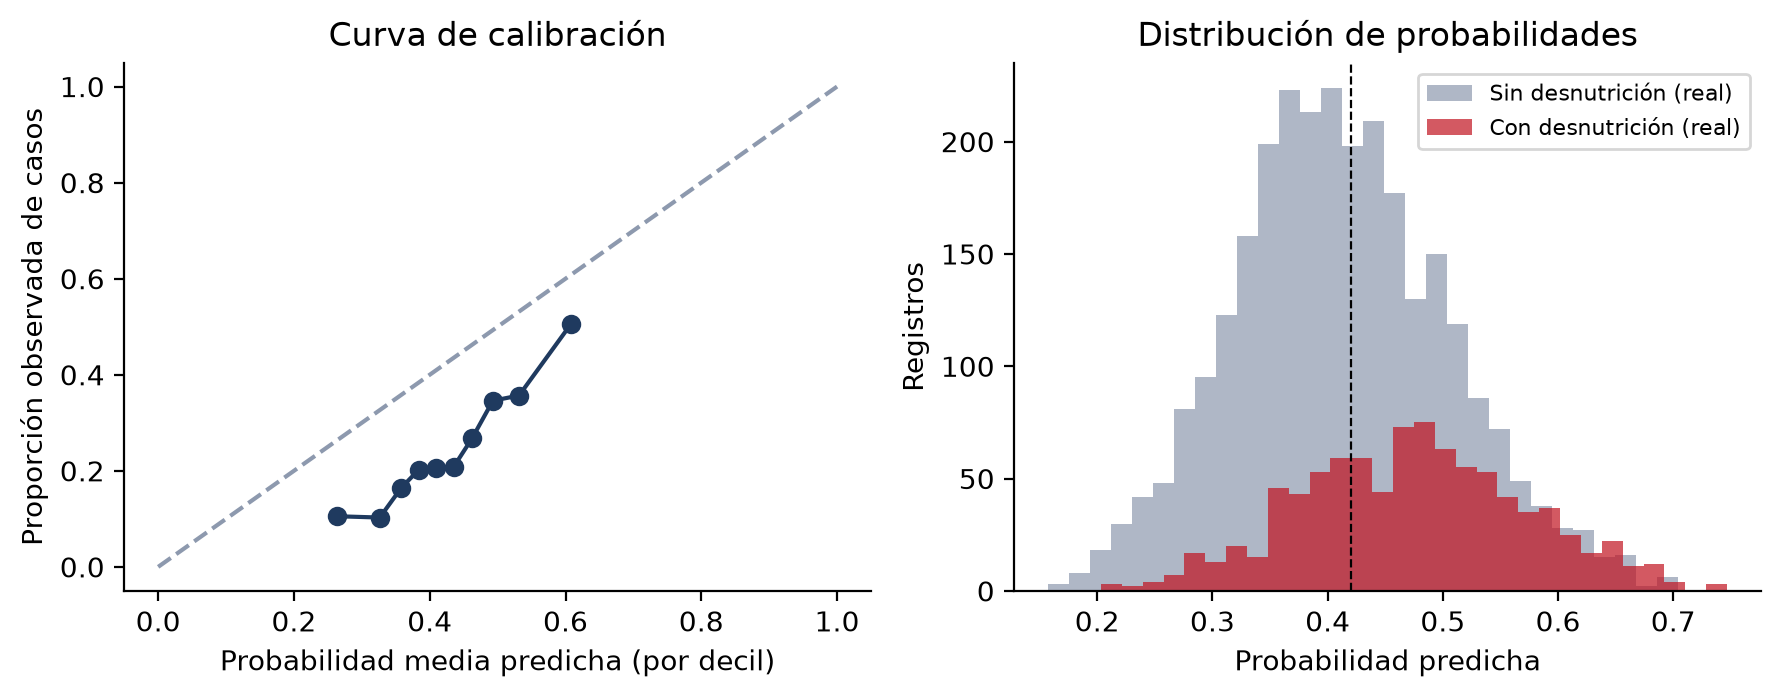
\includegraphics[width=0.95\textwidth]{figuras/anexo-calibracion.png}
  \caption{Curva de calibración y distribución de probabilidades predichas. Elaboración propia.}
  \label{fig:calibracion}
\end{figure}


\section*{H.4 Desempeño por subgrupos (detalle)}
\begin{table}[H]
  \caption{Desempeño por subgrupos en la prueba (umbral 0.42; IC de Wilson para la sensibilidad).}
  \label{tab:subgrupos}
  \tablabase\scriptsize
  \begin{tabular}{|l|c|c|c|c|c|c|c|}
    \hline
    \enc{Ámbito} & \enc{Variable} & \enc{Valor} & \enc{n} & \enc{Casos} & \enc{Sensibilidad (IC 95\,\%)} & \enc{Espec.} & \enc{ROC-AUC} \\ \hline
    Nacional & area & Rural & 1456 & 432 & 0.880 (0.846--0.907) & 0.312 & 0.682 \\ \hline
    Nacional & area & Urbano & 2243 & 480 & 0.525 (0.480--0.569) & 0.687 & 0.656 \\ \hline
    Tungurahua & area & Rural & 26 & 14 & 0.786 (0.524--0.924) & 0.083 & 0.423 \\ \hline
    Tungurahua & area & Urbano & 86 & 21 & 0.619 (0.409--0.792) & 0.662 & 0.686 \\ \hline
    Nacional & sexo & Hombre & 1904 & 510 & 0.720 (0.679--0.757) & 0.514 & 0.672 \\ \hline
    Nacional & sexo & Mujer & 1795 & 402 & 0.659 (0.612--0.704) & 0.586 & 0.679 \\ \hline
    Tungurahua & sexo & Hombre & 46 & 13 & 0.769 (0.497--0.918) & 0.424 & 0.608 \\ \hline
    Tungurahua & sexo & Mujer & 66 & 22 & 0.636 (0.430--0.803) & 0.682 & 0.718 \\ \hline
    Nacional & edad (meses) & 0-5 & 294 & 64 & 0.609 (0.487--0.719) & 0.504 & 0.597 \\ \hline
    Nacional & edad (meses) & 6-11 & 370 & 85 & 0.659 (0.553--0.751) & 0.540 & 0.650 \\ \hline
    Nacional & edad (meses) & 12-23 & 762 & 259 & 0.892 (0.848--0.924) & 0.247 & 0.654 \\ \hline
    Nacional & edad (meses) & 24-35 & 747 & 209 & 0.751 (0.688--0.805) & 0.493 & 0.667 \\ \hline
    Nacional & edad (meses) & 36-59 & 1526 & 295 & 0.505 (0.448--0.562) & 0.709 & 0.663 \\ \hline
    Tungurahua & edad (meses) & 12-23 & 26 & 10 & 0.800 (0.490--0.943) & 0.250 & 0.600 \\ \hline
    Tungurahua & edad (meses) & 24-35 & 21 & 8 & 0.750 (0.409--0.929) & 0.462 & 0.519 \\ \hline
    Tungurahua & edad (meses) & 36-59 & 54 & 13 & 0.538 (0.291--0.768) & 0.732 & 0.704 \\ \hline
  \end{tabular}
\end{table}


\section*{H.5 Hiperparámetros del modelo final}
\begin{table}[H]
  \caption{Hiperparámetros efectivos del Random Forest final.}
  \label{tab:hiper}
  \tablabase\scriptsize
  \begin{tabular}{|p{3.4cm}|p{2.6cm}|p{3.4cm}|p{2.6cm}|}
    \hline
    \enc{Parámetro} & \enc{Valor} & \enc{Parámetro} & \enc{Valor} \\ \hline
    \texttt{bootstrap} & True & \texttt{min\_samples\_split} & 2 \\ \hline
    \texttt{ccp\_alpha} & 0.0 & \texttt{min\_weight\_fraction\_leaf} & 0.0 \\ \hline
    \texttt{class\_weight} & balanced & \texttt{monotonic\_cst} & None \\ \hline
    \texttt{criterion} & gini & \texttt{n\_estimators} & 300 \\ \hline
    \texttt{max\_depth} & 20 & \texttt{n\_jobs} & None \\ \hline
    \texttt{max\_features} & sqrt & \texttt{oob\_score} & False \\ \hline
    \texttt{max\_leaf\_nodes} & None & \texttt{random\_state} & 42 \\ \hline
    \texttt{max\_samples} & None & \texttt{verbose} & 0 \\ \hline
    \texttt{min\_impurity\_decrease} & 0.0 & \texttt{warm\_start} & False \\ \hline
    \texttt{min\_samples\_leaf} & 10 &  &  \\ \hline
  \end{tabular}
\end{table}


\section*{H.6 Importancia de variables (30 principales)}
\begin{table}[H]
  \caption{Las 30 variables con mayor importancia (suma de sus columnas codificadas, \% del total).}
  \label{tab:top30}
  \tablabase\scriptsize
  \begin{tabular}{|c|p{6.4cm}|c|}
    \hline
    \enc{N.º} & \enc{Variable} & \enc{Importancia (\%)} \\ \hline
    1 & \texttt{edad\_meses} & 4.50 \\ \hline
    2 & \texttt{factor\_expansion} (diseño muestral) & 3.70 \\ \hline
    3 & \texttt{grupo\_edad\_meses} & 3.67 \\ \hline
    4 & \texttt{estrato} (diseño muestral) & 3.64 \\ \hline
    5 & \texttt{nivel\_instruccion\_madre} & 3.21 \\ \hline
    6 & \texttt{provincia} & 3.09 \\ \hline
    7 & \texttt{tamano\_recien\_nacido} & 2.75 \\ \hline
    8 & \texttt{peso\_nacer\_gramos} & 2.69 \\ \hline
    9 & \texttt{etnia\_madre} & 2.63 \\ \hline
    10 & \texttt{area} & 2.14 \\ \hline
    11 & \texttt{numero\_controles\_prenatales} & 2.07 \\ \hline
    12 & \texttt{region\_madre} & 2.02 \\ \hline
    13 & \texttt{semanas\_primer\_control} & 2.01 \\ \hline
    14 & \texttt{sexo} & 1.95 \\ \hline
    15 & \texttt{talla\_nacer\_cm} & 1.94 \\ \hline
    16 & \texttt{controles\_0\_1\_anio} & 1.94 \\ \hline
    17 & \texttt{lugar\_parto} & 1.75 \\ \hline
    18 & \texttt{tipo\_parto} & 1.66 \\ \hline
    19 & \texttt{lactancia\_meses} & 1.64 \\ \hline
    20 & \texttt{controles\_1\_2\_anios} & 1.59 \\ \hline
    21 & \texttt{personal\_parto} & 1.47 \\ \hline
    22 & \texttt{controles\_2\_5\_anios} & 1.45 \\ \hline
    23 & \texttt{lugar\_control\_prenatal} & 1.43 \\ \hline
    24 & \texttt{tiempo\_primer\_control\_nino} & 1.32 \\ \hline
    25 & \texttt{examen\_sifilis\_embarazo} & 1.30 \\ \hline
    26 & \texttt{vitamina\_a\_12\_meses} & 1.28 \\ \hline
    27 & \texttt{perimetro\_cefalico\_cm} & 1.23 \\ \hline
    28 & \texttt{corte\_oportuno\_cordon} & 1.21 \\ \hline
    29 & \texttt{desparasitacion\_6\_meses} & 1.11 \\ \hline
    30 & \texttt{control\_posparto} & 1.09 \\ \hline
  \end{tabular}
\end{table}


%% ----------------------------------------------------------------- ANEXO I
\anexo{I}{Código Esencial}

Se incluye el código esencial del pipeline y del servicio. El resto está en el repositorio (Anexo~E). Los comentarios conservan la redacción original del código.

\section*{I.1 Construcción de la base sin fuga (\texttt{build\_clean\_dataset.py})}
\lstinputlisting[language=Python,basicstyle=\ttfamily\scriptsize,frame=single]{anexos/codigo/build_clean_dataset.py}

\section*{I.2 Partición reproducible (\texttt{split\_dataset.py})}
\lstinputlisting[language=Python,basicstyle=\ttfamily\scriptsize,frame=single]{anexos/codigo/split_dataset.py}

\section*{I.3 Revisión de fuga por variable (\texttt{leakage\_screen.py})}
\lstinputlisting[language=Python,basicstyle=\ttfamily\scriptsize,frame=single]{anexos/codigo/leakage_screen.py}

\section*{I.4 Preprocesamiento, modelos, umbral y evaluación (\texttt{entrenar\_modelo.py}, extracto)}
\lstinputlisting[language=Python,basicstyle=\ttfamily\scriptsize,frame=single]{anexos/codigo/entrenar_extracto.py}

\section*{I.5 Servicio de predicción (\texttt{predictor.py})}
\lstinputlisting[language=Python,basicstyle=\ttfamily\scriptsize,frame=single]{anexos/codigo/predictor.py}

\section*{I.6 Ruta de predicción individual (\texttt{main.py}, extracto)}
\lstinputlisting[language=Python,basicstyle=\ttfamily\scriptsize,frame=single]{anexos/codigo/main_predict.py}
